% !TEX TS-program = lualatex
% Copyright (C)  2026 Alain Matthes
% This work may be distributed and/or modified under the
% conditions of the LaTeX Project Public License, either version 1.3
% of this license or (at your option) any later version.
% The latest version of this license is in
%   http://www.latex-project.org/lppl.txt
% and version 1.3 or later is part of all distributions of LaTeX
% version 2005/12/01 or later.
% This work has the LPPL maintenance status `maintained'.
% The Current Maintainer of this work is Alain Matthes

% TKZdoc-fn-main : documentation (American English) of tkz-fn.

\documentclass[DIV         = 14,
               fontsize    = 10,
               index       = totoc,
               twoside,
               headings    = small
               ]{tkz-doc}
\usepackage{etoc}
\gdef\tkznameofpack{tkz-fn}
\gdef\tkzversionofpack{1.00c}
\gdef\tkzdateofpack{2026/10/19}
\gdef\tkznameofdoc{doc-tkz-fn}
\gdef\tkzdateofdoc{2026/10/19}
\gdef\tkzversionofdoc{1.00c}
\gdef\tkzauthorofpack{Alain Matthes}
\gdef\tkzadressofauthor{}
\gdef\tkznamecollection{AlterMundus}
\gdef\tkzurlauthor{http://altermundus.fr}
\gdef\tkzurlauthorcom{http://altermundus.fr}
\gdef\tkzengine{lualatex}
\usepackage{tkz-tab}
\usepackage[english]{alterqcm}
\usepackage{tkz-fn}
\usetikzlibrary{arrows,patterns,shapes.geometric}
\usepackage[colorlinks]{hyperref}
\hypersetup{
      linkcolor=Gray,
      citecolor=Green,
      filecolor=Mulberry,
      urlcolor=NavyBlue,
      menucolor=Gray,
      runcolor=Mulberry,
      linkbordercolor=Gray,
      citebordercolor=Green,
      filebordercolor=Mulberry,
      urlbordercolor=NavyBlue,
      menubordercolor=Gray,
      runbordercolor=Mulberry,
      pdfsubject={Graph function with Lua},
      pdfauthor={\tkzauthorofpack},
      pdftitle={\tkznameofpack},
      pdfkeywords={tikz, pgf, lua, lualatex, graphic, maths, graph,
      function, tangent, area},
      pdfcreator={\tkzengine}
}
\usepackage{url}
\def\UrlFont{\small\ttfamily}

\usepackage{fontspec}
\setmainfont{texgyrepagella}[
  Extension = .otf,
  UprightFont = *-regular ,
  ItalicFont  = *-italic  ,
  BoldFont    = *-bold    ,
  BoldItalicFont = *-bolditalic ,
]
\setsansfont{texgyreheros}[
  Extension = .otf,
  UprightFont = *-regular ,
  ItalicFont  = *-italic  ,
  BoldFont    = *-bold    ,
  BoldItalicFont = *-bolditalic ,
]
\setmonofont{lmmono10-regular.otf}[
  Numbers={Lining,SlashedZero},
  ItalicFont=lmmonoslant10-regular.otf,
  BoldFont=lmmonolt10-bold.otf,
  BoldItalicFont=lmmonolt10-boldoblique.otf,
]
\newfontfamily\ttcondensed{lmmonoltcond10-regular.otf}
\linespread{1.05}
\usepackage{unicode-math}
\usepackage{fourier-otf}
\usepackage{tkzexample}
\usepackage{rotating,fancyvrb}
\usepackage[american]{babel}

\usepackage{microtype}
\usepackage[parfill]{parskip}
\usepackage{array,multirow,booktabs}
\usepackage{shortvrb}
\AtBeginDocument{\MakeShortVerb{\|}}

\RequirePackage{makeidx}
\makeindex
\colorlet{graphicbackground}{white}
\colorlet{codebackground}{Gray!10}
\def\blue{\color{blue}}
\def\red{\color{red}}
\begin{document}

%<--------------------- Première page présentation  ------------------------–>
\title{\tkznameofpack}
\date{\today}
\clearpage
\thispagestyle{empty}
\maketitle

\clearpage

\nameoffile{\tkznameofpack}

\defoffile{\textbf{tkz-fn.sty (v\tkzversionofpack)} is a package for drawing graphs of functions in 2D as simply as possible, with \TIKZ\ and Lua. It is the successor of \tkzname{tkz-fct}: \tkzname{gnuplot}, \tkzname{fp.sty} and \tkzname{tkz-base} are no longer needed, every computation is done by Lua and the document is compiled with \tkzname{LuaLaTeX}. The drawings are the kind used in high school mathematics; the presentation (French or American conventions, ``box'' axes as with \tkzname{pgfplots}) is chosen with options.}

\presentation

\vspace*{24pt}
\noindent\lefthand\ I would like to thank \tkzimp{Till Tantau} for the wonderful tool \tkzname{\TIKZ}, and \tkzimp{Michel Bovani} for the \tkzname{fourier} fonts.

\vspace*{12pt}
\noindent\lefthand\ I would also like to thank \tkzimp{David Arnold}, \tkzimp{Pablo González Luengo}, \tkzimp{Wolfgang Büchel}, \tkzimp{John Kitzmiller} and \tkzimp{Gaétan Marris} for their help with \tkzname{tkz-fct}; the examples of this documentation come from it.

\vspace*{12pt}
\noindent\lefthand\ You will find many examples on my website:
\href{http://altermundus.fr}{altermundus.fr}

\vfill
Please send your comments and bug reports to: \href{mailto:al.ma@mac.com}{\textcolor{blue}{Alain Matthes}}.

This work may be distributed and/or modified under the
conditions of the LaTeX Project Public License, either version 1.3
of this license or (at your option) any later version.
%<--------------------------------------------------------------------------->

\clearpage
\tableofcontents

\clearpage
\newpage

\setlength{\parskip}{1ex plus 0.5ex minus 0.2ex}
%<---------------------------- the files ------------------------------------>
\section{Overview}

\subsection{Why a new package?}

\tkzname{tkz-fct} delegated the computation of the points of the curves to \tkzname{gnuplot}, and the computation of values and slopes to \tkzname{fp.sty}. You had to install \tkzname{gnuplot}, allow \tkzname{shell-escape}, write each function with two syntaxes and often rewrite polynomials in \tkzimp{Horner} form to avoid the overflows of \tkzname{fp}.

\tkzname{tkz-fn} replaces all this with \tkzname{Lua}, which is part of \tkzname{LuaLaTeX}:
\begin{itemize}
  \item the points of the curves, the values, the derivatives and the areas are computed by Lua in double precision;
  \item a function is defined only once, with the syntax of Lua (|x^2|, |sin(x)|, |exp(x)|);
  \item no \tkzname{gnuplot}, no \tkzname{shell-escape}, no auxiliary file;
  \item \tkzname{tkz-fn} depends only on \TIKZ; it uses neither \tkzname{tkz-base} nor \tkzname{tkz-euclide};
  \item numerical results are written in the American or in the French way;
  \item the axes can be drawn as in school textbooks, with arrows at one or both ends, or as a ``box'' as with \tkzname{pgfplots};
  \item a bridge makes the points defined by \tkzname{tkz-fn} available to \tkzname{tkz-elements}.
\end{itemize}

All the macros begin with \tkzname{\textbackslash tkzFn}, so there is no conflict with \tkzname{tkz-fct}, \tkzname{tkz-base} or \tkzname{tkz-euclide}.

\subsection{Two coordinate spaces}

A coordinate system is defined with \tkzcname{tkzFnInit}, using the options \tkzname{xmin}, \tkzname{xmax}, \tkzname{xstep}, \tkzname{ymin}, \tkzname{ymax} and \tkzname{ystep}. \tkzname{xstep} is the value represented by one centimeter on the $x$-axis, \tkzname{ystep} the value represented by one centimeter on the $y$-axis.

\begin{itemize}
  \item Every computation is done in the units of the coordinate system: $f(x)$, the slope of a tangent line, an area, a Riemann sum, the coordinates of a point.
  \item The drawing is done in centimeters. The conversion happens at the last moment:
  \[ X = \frac{x}{\text{xstep}} \qquad Y = \frac{y}{\text{ystep}} \]
\end{itemize}

So you no longer write |\x| instead of |x| when \tkzname{xstep} is not 1. For example, let us draw the graph of the function $f$ defined by:

\[
 0\leq x\leq 100 \ \text{and}\ f(x)=x^3
\]

The values of $f(x)$ lie between 0 and $\tkzFnPrint{1000000}$. With \tkzname{xstep=10} and \tkzname{ystep=100000}, the axes are about $10$ cm long (without scaling).

\begin{tkzexample}[latex=10cm,small]
\begin{tikzpicture}[scale=.5]
  \tkzFnInit[xmax=100,xstep=10,
             ymin=0,ymax=1000000,
             ystep=100000,xmin=0]
  \tkzFnGrid
  \tkzFnAxes[decimals=0]
  \tkzFnDraw[color=red,
             domain=0:100]{x^3}
\end{tikzpicture}
\end{tkzexample}

\endinput

\section{Installation and compilation}

\subsection{Files}

The package consists of two files:
\begin{itemize}
  \item \tkzname{tkz-fn.sty}: the \LaTeX{} interface (macros and options);
  \item \tkzname{tkz\_fn.lua}: the Lua code (computations and generated \TIKZ\ code).
\end{itemize}

Both files must be placed in a folder known to \TeX{}, for example \tkzname{texmf/tex/latex/tkz-fn}, or in the folder of the document.

\subsection{Loading}

\begin{tkzltxexample}[]
\usepackage{tkz-fn}         % format according to the language of babel
\usepackage[us]{tkz-fn}     % American format of the results
\usepackage[fr]{tkz-fn}     % French format of the results
\end{tkzltxexample}

\TIKZ\ and its library \tkzname{plotmarks} are loaded automatically. Some \TIKZ\ options used in the examples need other libraries: |\usetikzlibrary{arrows,patterns}|.

\subsection{Compilation}

The document must be compiled with \tkzname{LuaLaTeX}. The \tkzname{shell-escape} option is not needed and no auxiliary file is created.

\subsection{Writing functions}

Expressions are Lua expressions. The variable is |x| for a function, |t| for a parametric or a polar curve.

\begin{center}
\begin{tabular}{lll}
\toprule
Lua & old syntax (gnuplot) & description \\
\midrule
|x^3|, |x^0.5| & |x**3|, |x**0.5| & power \\
|1/3| & |1./3| & quotient (always decimal) \\
|ln(x)| or |log(x)| & |log(x)| & natural logarithm \\
|log10(x)| & |log10(x)| & common logarithm \\
|exp(x)|, |e| & |exp(x)|, |exp(1)| & exponential, number $\text{e}$ \\
|sqrt(x)|, |abs(x)| & |sqrt(x)|, |abs(x)| & square root, absolute value \\
|sin|, |cos|, |tan| & same & radians \\
|asin|, |acos|, |atan| & same & inverse functions \\
|sinh|, |cosh|, |tanh| & same & hyperbolic functions \\
|pi| & |pi| & $\pi$ \\
|floor|, |ceil|, |sign|, |mod(a,b)| & |floor|, |ceil|, |sgn|, |%| & \\
|cbrt(x)|, |root(x,n)| & & cube root, $n$-th root \\
\bottomrule
\end{tabular}
\end{center}

\tkzHand A function defined with \tkzcname{tkzFnDef} can be used in another expression: |2*f(x)+1|. A global Lua variable can be used as a parameter: |\directlua{a = 0.5}| then |a*x^2|.

\tkzHand The functions |diff(f,x)|, |integral(f,a,b)| and |riemann(f,a,b,n,"left")| give the derivative at a point, the integral (Simpson's rule) and a Riemann sum. They are used with \tkzcname{tkzFnPrint}.

\tkzBomb An argument between parentheses must not contain an unprotected closing parenthesis: write |(f,{1/exp(1)})|, not |(f,1/exp(1))|.

\endinput

\section{The coordinate system}

These macros replace those of \tkzname{tkz-base} (\tkzcname{tkzInit}, \tkzcname{tkzGrid}, \tkzcname{tkzAxeXY}, \tkzcname{tkzDrawX}, \tkzcname{tkzClip}, \tkzcname{tkzRep}, \tkzcname{tkzText}).

\subsection{Initialization: \tkzcname{tkzFnInit}}

\begin{NewMacroBox}{tkzFnInit}{\oarg{options}}
\begin{tabular}{lll}
\toprule
options             & default & definition  \\
\midrule
\TOline{xmin}{-5}{smallest $x$}
\TOline{xmax}{5}{largest $x$}
\TOline{xstep}{1}{value represented by 1 cm on the $x$-axis}
\TOline{ymin}{-5}{smallest $y$}
\TOline{ymax}{5}{largest $y$}
\TOline{ystep}{1}{value represented by 1 cm on the $y$-axis}
\TOline{xorigin}{0}{$x$ placed at $X=0$ (a year, for example)}
\TOline{yorigin}{0}{$y$ placed at $Y=0$}
\TOline{enlarge}{0 (0.1 without value)}{enlarges the window by a fraction of its size}
\TOline{enlarge x, enlarge y}{enlarge}{enlargement in one direction only}
\bottomrule
\end{tabular}

\emph{Values can be expressions: \texttt{xmax=2*pi}.}
\end{NewMacroBox}

\subsection{Grid: \tkzcname{tkzFnGrid}}

\begin{NewMacroBox}{tkzFnGrid}{\oarg{options}\parg{$x_1$,$y_1$}\parg{$x_2$,$y_2$}}
\emph{The region is optional; by default the grid covers the window.}

\begin{tabular}{lll}
\toprule
options             & default & definition  \\
\midrule
\TOline{dx}{xstep}{distance between two vertical lines}
\TOline{dy}{ystep}{distance between two horizontal lines}
\TOline{sub}{false}{adds a subgrid}
\TOline{subdx}{dx/5}{spacing of the subgrid}
\TOline{subdy}{dy/5}{spacing of the subgrid}
\bottomrule
\end{tabular}

\emph{Other options are \TIKZ\ options; the style is \tkzname{tkzfn grid}.}
\end{NewMacroBox}

\begin{tkzexample}[latex=8cm]
\begin{tikzpicture}[scale=1.25]
 \tkzFnInit[xmin=-2,xmax=3,
            ymin=-1,ymax=2]
 \tkzFnGrid[sub,color=orange]
 \tkzFnAxes
\end{tikzpicture}
\end{tkzexample}

\subsection{Axes: \tkzcname{tkzFnAxes}, \tkzcname{tkzFnAxisX}, \tkzcname{tkzFnAxisY}}

\begin{NewMacroBox}{tkzFnAxes}{\oarg{options}}
\emph{Draws both axes, the tick marks and their labels. The axes cross at $(0, 0)$ if this point is in the window, at $(x_{\min}, y_{\min})$ otherwise. Values are written in the American or the French way (section~\ref{sec:format}).}

\begin{tabular}{lll}
\toprule
options             & default & definition  \\
\midrule
\TOline{dx, dy}{xstep, ystep}{distance between two tick marks}
\TOline{xlabel, ylabel}{\$x\$, \$y\$}{names of the axes}
\TOline{ticks}{true}{tick marks}
\TOline{labels}{true}{tick labels}
\TOline{line}{true}{axis lines}
\TOline{origin}{0 or O}{label of the origin (0 American, O French)}
\TOline{trig}{0}{if $n>0$, ticks of the $x$-axis at multiples of $\pi/n$}
\TOline{decimals}{4}{maximum number of decimal places}
\TOline{arrows}{end}{arrows: \texttt{end}, \texttt{both} or \texttt{none} (section~\ref{sec:arrows})}
\TOline{box}{false}{``box'' axes (section~\ref{sec:box})}
\TOline{style}{school}{\texttt{school} or \texttt{box}}
\TOline{tick length}{3pt}{length of the tick marks (box)}
\bottomrule
\end{tabular}

\emph{\tkzcname{tkzFnAxisX} and \tkzcname{tkzFnAxisY} draw a single axis; their options are the same with \tkzname{label}, \tkzname{label style} and \tkzname{step} instead of \tkzname{xlabel}, \tkzname{ylabel} and \tkzname{dx}. With \tkzname{ticks=false}, you get the equivalent of \tkzcname{tkzDrawX}.}
\end{NewMacroBox}

\begin{tkzexample}[latex=8cm]
\begin{tikzpicture}
  \tkzFnInit[xmin=-7,xmax=7,
             ymin=-1,ymax=1]
  \tkzFnAxisY
  \tkzFnAxisX[trig=2]
  \tkzFnDraw[red]{sin(x)}
\end{tikzpicture}
\end{tkzexample}

\subsection{Clipping: \tkzcname{tkzFnClip}}

\begin{NewMacroBox}{tkzFnClip}{\oarg{margin in pt}}
\emph{Restricts the rest of the drawing to the window (enlarged by a margin). As with \tkzcname{clip}, use it preferably inside a \tkzname{scope} environment. Curves and tangent lines are clipped to the window anyway (option \tkzname{clip}).}
\end{NewMacroBox}

\subsection{Unit vectors: \tkzcname{tkzFnRep}}

\begin{NewMacroBox}{tkzFnRep}{\oarg{\TIKZ\ options}}
\emph{Draws the vectors $\vec{\imath}$ and $\vec{\jmath}$; the style is \tkzname{tkzfn rep}.}
\end{NewMacroBox}

\subsection{Text: \tkzcname{tkzFnText}}

\begin{NewMacroBox}{tkzFnText}{\oarg{\TIKZ\ options}\parg{$x$,$y$}\marg{text}}
\emph{Places a text at the point with coordinates $(x, y)$ in the coordinate system. You can also give the name of a point: \tkzcname{tkzFnText}\texttt{[above](A)\{text\}}.}
\end{NewMacroBox}

\begin{tkzexample}[latex=8cm]
\begin{tikzpicture}[scale=1.5]
 \tkzFnInit[xmin=-3,xmax=3,
            ymin=-1,ymax=4]
 \tkzFnGrid[sub,subdx=.5,subdy=.5]
 \tkzFnAxes
 \tkzFnDraw[domain=-3:2]{(2-x)*exp(x)}
 \tkzFnText(-2,1.25){$\mathcal{C}_{f}$}
 \tkzFnRep
\end{tikzpicture}
\end{tkzexample}

\subsection{Arrows at both ends: \tkzname{arrows}}\label{sec:arrows}

In the United States, textbooks and graphing calculators often put an arrow at each end of the axes. The option \tkzname{arrows} of \tkzcname{tkzFnAxes}, \tkzcname{tkzFnAxisX} and \tkzcname{tkzFnAxisY} chooses the arrows:
\begin{itemize}
  \item \texttt{end} (default): one arrow at the positive end;
  \item \texttt{both}: an arrow at each end;
  \item \texttt{none}: no arrow.
\end{itemize}
|\tkzFnSetup{arrows=both}| chooses the arrows for all the following coordinate systems. The shape of the arrow tips is given by the style \tkzname{tkzfn axis}.

\begin{tkzexample}[latex=7cm]
\begin{tikzpicture}[scale=.6]
  \tkzFnInit[xmin=-5,xmax=5,
             ymin=-4,ymax=6]
  \tkzFnGrid
  \tkzFnAxes[arrows=both]
  \tkzFnDraw[blue,thick,<->,>=stealth,
             clip=false,domain=-4.2:4.2]{x^2/2-3}
\end{tikzpicture}
\end{tkzexample}

For a whole document, with other arrow tips:

\begin{tkzexample}[latex=7cm]
\tkzFnSetup{arrows=both}
\tikzset{tkzfn axis/.style={>=latex}}
\begin{tikzpicture}[scale=.7]
  \tkzFnInit[xmin=-2,xmax=3,xstep=.5,
             ymin=-1.5,ymax=1.5,ystep=.5]
  \tkzFnGrid[sub]
  \tkzFnAxes[dx=1]
  \tkzFnDraw[red,thick]{x^3/3-x}
\end{tikzpicture}
\tkzFnSetup{arrows=end}
\tikzset{tkzfn axis/.style={->,>=stealth}}
\end{tkzexample}

Without arrows:

\begin{tkzexample}[latex=7cm]
\begin{tikzpicture}[scale=.6]
  \tkzFnInit[xmin=-1,xmax=5,
             ymin=-1,ymax=3]
  \tkzFnAxes[arrows=none]
  \tkzFnDraw{sqrt(x)}
\end{tikzpicture}
\end{tkzexample}

\newpage
\subsection{``Box'' axes: \tkzname{box}}\label{sec:box}

This presentation is usual in scientific publications and with \tkzname{pgfplots}, and less common in high school textbooks. With \tkzname{pgfplots} it is obtained with the \tkzname{axis} environment; with \tkzname{tkz-fn} an option is enough:

\begin{itemize}
  \item |\tkzFnAxes[box]|: a frame surrounds the window, the tick marks point inward on the four sides, every value (including those at the edges) is written outside, there is no arrow and no origin label;
  \item the names of the axes are written only when they are given: |xlabel| below the frame, |ylabel| on the left, vertically;
  \item |\tkzFnSetup{axes=box}| chooses this presentation for all the following coordinate systems; |\tkzFnSetup{axes=school}| comes back to the usual one;
  \item the option \tkzname{mark} of \tkzcname{tkzFnDraw} puts a mark at each computed point (\tkzname{samples} sets their number);
  \item the option \tkzname{enlarge} of \tkzcname{tkzFnInit} moves the curve away from the frame; the default domain is still $[x_{\min}, x_{\max}]$.
\end{itemize}

The style of the frame is \tkzname{tkzfn box}. The following examples reproduce a figure made with \tkzname{pgfplots}.

\begin{tkzexample}[latex=7cm]
\tkzFnDef{f}{1/((1e9*x/11.778)*3.273e-8
              -3.273e-8+1)}
\begin{tikzpicture}[scale=.9]
  \tkzFnInit[xmin=0,xmax=6,
             ymin=0,ymax=1,ystep=.2]
  \tkzFnAxes[box]
  \tkzFnDraw[blue,mark=*,mark size=1.5pt,
             samples=13,domain=0:5](f)
  \tkzFnDrawData[red,mark=square*,
                 mark size=1.5pt]{.125/.744}
\end{tikzpicture}
\end{tkzexample}

The default domain is $[x_{\min}, x_{\max}]$:

\begin{tkzexample}[latex=7cm]
\begin{tikzpicture}[scale=.9]
  \tkzFnInit[xmin=0,xmax=6,
             ymin=0,ymax=1,ystep=.2]
  \tkzFnAxes[box]
  \tkzFnDraw[blue,mark=*,mark size=1.5pt,
             samples=25](f)
  \tkzFnDrawData[red,mark=square*,
                 mark size=1.5pt]{.125/.744}
\end{tikzpicture}
\end{tkzexample}

With \tkzname{enlarge} (10\,\% by default) and the names of the axes:

\begin{tkzexample}[latex=7cm]
\begin{tikzpicture}[scale=.9]
  \tkzFnInit[xmin=0,xmax=6,ymin=0,ymax=1,
             ystep=.2,enlarge]
  \tkzFnAxes[box,xlabel=$x$,
             ylabel=$f(x)$]
  \tkzFnDraw[blue,mark=*,mark size=1.5pt,
             samples=25](f)
  \tkzFnDrawData[red,mark=square*,
                 mark size=1.5pt]{.125/.744}
\end{tikzpicture}
\end{tkzexample}

\newpage
With |\tkzFnSetup{axes=box}|, the grid and the ticks at multiples of $\pi$ are used as usual; the option \tkzname{smooth} is passed to \TIKZ.

\begin{tkzexample}[vbox]
\tkzFnSetup{axes=box}
\begin{tikzpicture}[scale=.6]
  \tkzFnInit[xmin=-3,xmax=3,ymin=0,ymax=20000,ystep=4000]
  \tkzFnGrid
  \tkzFnAxes[xlabel=$t$,ylabel=Population]
  \tkzFnDraw[red,thick,smooth,samples=7]{2000*x^2}
\end{tikzpicture}\qquad
\begin{tikzpicture}[scale=.6]
  \tkzFnInit[xmin=-7,xmax=7,ymin=-1,ymax=1,ystep=.5]
  \tkzFnAxes[trig=2]
  \tkzFnDraw{sin(x)}
\end{tikzpicture}
\tkzFnSetup{axes=school}
\end{tkzexample}

\endinput

\section{Drawing a function}

Lua computes the points needed to draw the curve. Their number is set by the option \tkzname{samples}. \TIKZ\ then draws the line through these points.

\subsection{Defining a function: \tkzcname{tkzFnDef}}

\begin{NewMacroBox}{tkzFnDef}{\marg{name}\marg{expression}}
\emph{Defines a function of the variable \texttt{x}. The name is a Lua name (letters, digits, \texttt{\_}). The function is then referred to by its name in every macro: \tkzcname{tkzFnDraw}\texttt{(f)}, \tkzcname{tkzFnTangent}\texttt{(f,1)}, \tkzcname{tkzFnArea}\texttt{(f)}, etc. In Lua, it is stored in the table \texttt{FN}: \texttt{FN.f(2)}.}

\begin{tabular}{lll}
\toprule
arguments             & example & explanation  \\
\midrule
\TAline{name}{f}{name of the function}
\TAline{expression}{x\string^3-2*x}{Lua expression in x}
\bottomrule
\end{tabular}
\end{NewMacroBox}

\subsection{Drawing a function: \tkzcname{tkzFnDraw}}

\begin{NewMacroBox}{tkzFnDraw}{\oarg{options}\parg{name} \textrm{or} \oarg{options}\marg{expression}}
\emph{The function is given by its name, or directly by its expression; the option \tkzname{name} then gives it a name.}

\begin{tabular}{lll}
\toprule
options             & default & definition     \\
\midrule
\TOline{domain}{xmin:xmax}{domain of the drawing}
\TOline{samples}{200}{number of computed points}
\TOline{name}{}{name given to the function}
\TOline{clip}{true}{the curve is clipped to the window}
\TOline{mark=\dots}{}{a mark at each computed point (\tkzname{plotmarks})}
\TOline{smooth}{}{curve smoothed by \TIKZ}
\bottomrule
\end{tabular}

\emph{Other options are \TIKZ\ options; the style is \tkzname{tkzfn curve}.}
\end{NewMacroBox}

\tkzHand The coordinate system must be initialized with \tkzcname{tkzFnInit} before \tkzcname{tkzFnDraw} is used.

\tkzHand The curve is interrupted where the function is not defined (|ln(x)| for $x\leq 0$) and where it jumps from one side of the window to the other (vertical asymptote).

%<--------------------------------------------------------------------------->
\subsection{Option: \tkzname{samples}}

Two points are enough to draw a line: \tkzname{samples=2}. Here 400 points are requested; the default value is 200.

\begin{tkzexample}[latex=7cm]
\begin{tikzpicture}[scale=1]
    \tkzFnInit[xmin=0,xmax=5,
               ymin=0,ymax=2]
    \tkzFnGrid[sub]
    \tkzFnAxes
    \tkzFnDraw[samples=400,
               domain=.5:5]{1/x}
\end{tikzpicture}
\end{tkzexample}

%<--------------------------------------------------------------------------->
\subsection{Options: \tkzname{xstep, ystep}}

\begin{tkzexample}[]
\begin{tikzpicture}
\tkzFnInit[xmin=0,xmax=110,xstep=10,
           ymin=0,ymax=6,ystep=1]
\tkzFnAxisX[label={\textit{Age}},
            label style={below=12pt,left}]
\tkzFnAxisY[label={\textit{Liters}}]
\tkzFnDraw[domain=0.1:100]{50/x}
\end{tikzpicture}
\end{tkzexample}

\subsection{Changing \tkzname{xstep} and \tkzname{ystep}}

This time the domain goes from 0 to 700 and the values of the function from $0$ to $\tkzFnPrint{1200}$. With \tkzname{tkz-fct}, you had to write |\x| instead of $x$ and |1./90000| instead of |1/90000|; this is no longer necessary.

\begin{tkzexample}[vbox]
\begin{tikzpicture}[scale=1.5]
 \tkzFnInit[xmin=0,xmax=700,xstep=100,
            ymin=0,ymax=1200,ystep=400]
 \tkzFnGrid(0,0)(700,1200)  \tkzFnAxes
 \tkzFnDraw[color=red,samples=100,line width=0.8pt,domain=0:700]
        {(1/90000)*x^3-(1/100)*x^2+(113/36)*x}
\end{tikzpicture}
\end{tkzexample}

\subsection{\tkzname{ystep} and constant functions}

With \tkzname{gnuplot}, |80/6| was an integer division and you had to write |80.|; with Lua, computations are always done with decimal numbers.

\begin{tkzexample}[vbox]
 \begin{tikzpicture}[scale=0.4]
 \tkzFnInit[xmin=0,xmax=30,ymin=0,ymax=90,ystep=6]
 \tkzFnAxisX[ticks=false,label=$t$]
 \tkzFnAxisY[ticks=false,label=$P$]
 \tkzFnDraw[line width=1pt,color=red,dashed,domain=0:30]{80}
 \tkzFnDraw[line width=1pt,color=blue,domain=0:30]{80/(1+4*exp(-0.21*x))}
 \tkzFnText[above,color=red](20,80){$P=80$}
\end{tikzpicture}
\end{tkzexample}

\subsection{Linear functions}
Two points are enough to draw a line: \tkzname{samples=2}.

\begin{tkzexample}[vbox]
 \begin{tikzpicture}[]
 \tkzFnInit[xmin=0,xmax=10,ymin=0,ymax=20,ystep=5]
 \tkzFnAxes
 \tkzFnDraw[color=red,domain=0:10,samples=2]{2*x+5}
 \tkzFnDraw[color=blue,domain=0:10,samples=2]{-x+15}
 \tkzFnDraw[color=green,domain=0:10,samples=2]{7}
\end{tikzpicture}
\end{tkzexample}

%<--------------------------------------------------------------------------->
\subsection{Subgrid}

   $y=(x-4)\text{e}^{-0.25x+5}$

Another grid can be drawn on a part of the window.

\begin{tkzexample}[latex=8cm]
\begin{tikzpicture}[scale=.8]
 \tkzFnInit[xmin=4,xmax=18,xstep=2,
            ymin=20,ymax=90,ystep=10]
 \tkzFnDraw[domain=5:18]
        {(x-4)*exp(-0.25*x+5)}
 \tkzFnGrid(4,20)(18,90)
 \tkzFnAxes
 \tkzFnGrid[sub,
            subdx=0.5,
            subdy=2,
            color=brown](6,60)(12,90)
\end{tikzpicture}
\end{tkzexample}

%<--------------------------------------------------------------------------->
\subsection{Text and points}

\begin{center}
\begin{tkzexample}[vbox]
\begin{tikzpicture}[scale=2]
 \tkzFnInit[xmin=-3,xmax=3,ymin=-1,ymax=4]
 \tkzFnGrid[sub,subdx=.5,subdy=.5]
 \tkzFnAxes
 \tkzFnDraw[domain=-3:2]{(2-x)*exp(x)}
 \tkzFnText(-2,1.25){$\mathcal{C}_{f}$}
 \tkzFnDefPointXY[draw](2,0){A}
 \tkzFnLabelPoints(A)
\end{tikzpicture}
\end{tkzexample}
\end{center}

\endinput

\section{Points}

\subsection{A point on a curve: \tkzcname{tkzFnDefPoint}}

\begin{NewMacroBox}{tkzFnDefPoint}{\oarg{options}\parg{name of the function,$x$}\marg{name of the point}}
\emph{Computes the value of the function at $x$ and defines the point $(x, f(x))$. The point is a \TIKZ\ coordinate: it is then used by its name. If \tkzname{tkz-elements} is loaded, the point is also stored in the table \texttt{z} (section~\ref{sec:elements}).}

\medskip
\begin{tabular}{lll}
 \toprule
 arguments             & example & explanation                         \\
 \midrule
 \TAline{function,x}{(f,0.5)}{point of the graph of $f$ with $x=0.5$}
 \TAline{name of the point}{A}{name of the coordinate}
 \bottomrule
\end{tabular}

\begin{tabular}{lll}
 options             & default & explanation                         \\
 \midrule
 \TOline{draw}{false}{the point is drawn}
 \TOline{size}{1.5pt}{radius of the point}
 \bottomrule
\end{tabular}

\emph{Other options are \TIKZ\ options used to draw the point.}
\end{NewMacroBox}

\begin{NewMacroBox}{tkzFnDefPointXY}{\oarg{options}\parg{$x$,$y$}\marg{name of the point}}
\emph{Defines a point by its coordinates in the coordinate system (equivalent of \tkzcname{tkzDefPoint}).}
\end{NewMacroBox}

\begin{NewMacroBox}{tkzFnDrawPoints}{\oarg{options}\parg{A,B,\dots}}
\emph{Draws points; the option \tkzname{size} gives the radius, other options are \TIKZ\ options. The style is \tkzname{tkzfn point}; it replaces \tkzcname{tkzSetUpPoint}: }

|\tikzset{tkzfn point/.style={draw=black,fill=yellow}}|
\end{NewMacroBox}

\begin{NewMacroBox}{tkzFnLabelPoints}{\oarg{options}\parg{A,B,\dots}}
\emph{Writes the names of the points; \tkzcname{tkzFnLabelPoint}\texttt{[options](A)\{text\}} writes any text. Default position: \tkzname{above right}.}
\end{NewMacroBox}

\subsection{Example}

\begin{center}
\begin{tkzexample}[vbox]
\begin{tikzpicture}[scale=1.25]
  \tkzFnInit[xmin=-2,xmax=2,xstep=1,
             ymin=-8,ymax=24,ystep=8]
  \tkzFnGrid  \tkzFnAxes
  \tkzFnDraw[name=f,domain=-1.5:1]{3-1.3125*x^5-2.5*x^3}
  \tkzFnDefPoint(f,.5){A}  \tkzFnDrawPoints(A)
  \tkzFnLabelPoint[above right](A){$A_0$}
\end{tikzpicture}
\end{tkzexample}
\end{center}

\subsection{Option \tkzname{draw}}
The point is defined and drawn at once.

\begin{tkzexample}[latex=7cm,small]
\begin{tikzpicture}[scale=1.25]
  \tkzFnInit[xmin=-2,xmax=2,xstep=1,
             ymin=-8,ymax=24,ystep=8]
  \tkzFnGrid
  \tkzFnAxes
  \tkzFnDraw[name=f,domain=-1.5:1]
            {3-1.3125*x^5-2.5*x^3}
  \tkzFnDefPoint[draw,red,size=2pt](f,.5){A}
  \tkzFnLabelPoint[above right](A){$a$}
\end{tikzpicture}
\end{tkzexample}

\newpage
\subsection{Points without the curve: \tkzcname{tkzFnMarkPoints}}

With \tkzname{tkz-fct}, you had to define the macro \tkzcname{tkzFctLast} with the syntax of \tkzname{fp}. Now it is enough to define the function without drawing it.

\begin{NewMacroBox}{tkzFnMarkPoints}{\oarg{options}\parg{name of the function}\marg{list of $x$ values}}
\emph{Draws the points of the graph for the given values of $x$; the list is written as with \tkzcname{foreach}: \texttt{-1.5,-1.4,...,1}. The points have no name.}
\end{NewMacroBox}

\begin{tkzexample}[]
\begin{tikzpicture}[xscale=3,yscale=2]
  \tkzFnInit[xmin=-2,xmax=2,xstep=1,
             ymin=-8,ymax=24,ystep=8]
  \tkzFnGrid
  \tkzFnAxes
  \tkzFnDef{f}{3-1.3125*x^5-2.5*x^3}
  \tkzFnMarkPoints(f){-1.5,-1.4,...,1}
\end{tikzpicture}
\end{tkzexample}

\newpage
\subsection{Points without worrying about coordinates}

The domain goes from 0 to 800 and the values of the function from $0$ to $\tkzFnPrint{2000}$. The values of $x$ are given in the units of the coordinate system.

\begin{tkzexample}[]
\begin{tikzpicture}[scale=1.6]
  \tkzFnInit[xmin  = 0,  xmax  = 800,
             ymin  = 0,  ymax  = 2000,
             xstep = 100,ystep = 400]
  \tkzFnGrid
  \tkzFnAxes
  \tkzFnDraw[name   = f,
             color  = blue,
             domain = 0:800]
        {(1/90000)*x^3-(1/100)*x^2+(113/36)*x}
  \tkzFnMarkPoints(f){0,450,800}
\end{tikzpicture}
\end{tkzexample}

\newpage
\subsection{Points with two functions}

Each function has a name: there is no longer a \tkzname{with} option.

\begin{tkzexample}[vbox]
\begin{tikzpicture}[scale=4]
  \tkzFnInit[xmin=0,xmax=3,ymin=0,ymax=2]
  \tkzFnAxes
  \tkzFnGrid(0,0)(3,2)
  \tkzFnDraw[name=f,color=red,domain=1/3:3]
            {0.125*(3*x-1)+0.375*(3*x-1)/(x*x)}
  \tkzFnDraw[name=g,color=green,domain=1/3:3]{0.125*(3*x-1)}
  \tikzset{tkzfn point/.style={draw=black,fill=lightgray}}
  \tkzFnMarkPoints[size=2pt](f){1,2,3}
  \tkzFnMarkPoints[size=2pt](g){1/3,3}
  \tkzFnText[draw,color=red,fill=red!20](1,1.5)
          {$f(x)=\frac{1}{8}(3x-1)+\frac{3}{8}
           \left(\frac{3x-1}{x^2}\right)$}
  \tkzFnText[draw,color=green!50!black,fill=green!20]
               (2,0.3){$g(x)=\frac{1}{8}(3x-1)$}
\end{tikzpicture}
\end{tkzexample}

\subsection{Coordinates of a point: \tkzcname{tkzFnShowCoord} and \tkzcname{tkzFnPrintCoord}}

\begin{NewMacroBox}{tkzFnShowCoord}{\oarg{options}\parg{A}}
\emph{Draws the segments from the point to the axes and writes its coordinates (American or French format). The options \tkzname{xlabel} and \tkzname{ylabel} replace the computed values; with \tkzname{xlabel=false}, nothing is written. The style is \tkzname{tkzfn show coord}.}
\end{NewMacroBox}

\begin{NewMacroBox}{tkzFnPrintCoord}{\oarg{decimals}\parg{A}}
\emph{Writes the coordinates of the point in the text.}
\end{NewMacroBox}

\begin{tkzexample}[latex=7cm]
\begin{tikzpicture}[scale=1.2]
  \tkzFnInit[xmin=0,xmax=3,ymin=0,ymax=4]
  \tkzFnAxes
  \tkzFnDraw[name=f,domain=0:2.5]{x^2/2+1}
  \tkzFnDefPoint[draw](f,1.5){A}
  \tkzFnShowCoord(A)
  \tkzFnDefPoint[draw](f,2){B}
  \tkzFnShowCoord[xlabel=$b$,
                  ylabel=$f(b)$](B)
\end{tikzpicture}

$A\tkzFnPrintCoord(A)$
\end{tkzexample}

\endinput

\section{Naming the curves}

It is useful to give a name to the curves. Let us take as an example the function $f$ defined by:

\[
   x>0\ \text{and}\ f(x)=\dfrac{x^2+x-1}{x^3}
\]

A title is easily written with the macro \tkzcname{tkzFnText}. The coordinates are given in the units of the axes. To place a text along the curve, the simplest way is to define a point of the curve and to use its name.

\begin{tkzltxexample}[num]
  \tkzFnDefPoint(f,3){P}
  \tkzFnText[above right](P){${\mathcal{C}}_f$}
\end{tkzltxexample}

The first line defines the point $P$ of the graph with $x=3$. The second one places the text at $P$. The \TIKZ\ options refine the result.

\subsection{Adding a label}

\begin{center}
\begin{tkzexample}[vbox]
\begin{tikzpicture}
  \tkzFnInit[xmin=0,xmax=10,
             ymin=0,ymax=1.2,ystep=0.2]
  \tkzFnGrid
  \tkzFnAxes
  \tkzFnDraw[name=f,thick,color=red,domain=0.55:10]{(x*x+x-1)/x^3}
  \tkzFnText(3,-0.3){\textbf{Graph of} $\mathbf{f}$}
  \tkzFnDefPoint(f,3){P}
  \tkzFnText[above right,text=red](P){${\mathcal{C}}_f$}
\end{tikzpicture}
\end{tkzexample}
\end{center}

\endinput

\section{Tangent lines}

The slope is computed by Lua in the units of the coordinate system, so a tangent line is correct even when \tkzname{xstep} and \tkzname{ystep} are different. Each tangent line is made of two half-lines: on the left (l) and on the right (r). Their lengths are given by \tkzname{kl} and \tkzname{kr}, in units of the $x$-axis: the right half goes from the point of tangency $(a, f(a))$ to the point $(a+k_r, f(a)+k_r f'_+(a))$. With $kl=0$ or $kr=0$, the corresponding half is not drawn.

If the function is not differentiable at $a$, the two halves have different slopes; they are computed separately.

\subsection{Drawing a tangent line: \tkzcname{tkzFnTangent}}

\begin{NewMacroBox}{tkzFnTangent}{\oarg{options}\parg{name of the function,$a$}}
\begin{tabular}{lll}
 \toprule
 arguments             & example & explanation    \\
 \midrule
 \TAline{function,a}{(f,0)}{tangent line at the point with $x=0$}
 \bottomrule
\end{tabular}

\begin{tabular}{lll}
\toprule
options             & default & definition                         \\
\midrule
\TOline{draw}{false}{the point of tangency is drawn}
\TOline{kl}{1}{length of the left half (units of the $x$-axis)}
\TOline{kr}{1}{length of the right half}
\TOline{clip}{true}{the line is clipped to the window}
\bottomrule
\end{tabular}

\emph{Other options are \TIKZ\ options; the style is \tkzname{tkzfn tangent}, empty by default. To get the arrows of \tkzname{tkz-fct}:}

|\tikzset{tkzfn tangent/.style={->,>=latex}}|
\end{NewMacroBox}

\tkzHand The function does not need to be drawn; it only has to be defined.

%<--------------------------------------------------------------------------->
\subsection{Tangent line when \tkzname{xstep} and \tkzname{ystep} are not 1}

No computation is needed: just use the values of the tick marks.

\begin{tkzexample}[vbox]
\begin{tikzpicture}[xscale=1.5]
 \tkzFnInit[xmin=0,xmax=800,xstep=100,
            ymin=0,ymax=1800,ystep=400]
 \tkzFnGrid[color=brown,sub,subdx=50,subdy=200](0,0)(800,1800)
 \tkzFnAxes
 \tkzFnDraw[name=f,color=red,samples=100,domain=0:800]
    {(1/90000)*x^3-(1/100)*x^2+(113/36)*x}
 \tkzFnTangent[draw,color=blue,kr=300,kl=450](f,450)
 \tkzFnText[draw,color=black,fill=brown!50,opacity=0.8](300,1200)
 {$f(x)=\dfrac{1}{90000}x^3 -\dfrac{1}{{100}}x^2 +\dfrac{113}{36}x$}
\end{tikzpicture}
\end{tkzexample}

The slope at $450$ is $\tkzFnPrint[4]{diff(f,450)}$; it is obtained with |\tkzFnPrint[4]{diff(f,450)}|.

%<--------------------------------------------------------------------------->
\subsection{The options \tkzname{kl}, \tkzname{kr} and \tkzname{draw}}

\begin{tkzexample}[]
\begin{tikzpicture}[scale=1.5]
  \tikzset{tkzfn tangent/.style={->,>=latex}}
  \tkzFnInit[xmin=-3,xmax=4,ymin=-4,ymax=2]
  \tkzFnGrid  \tkzFnAxes[ticks=false]
  \tkzFnDraw[name=f,domain=-2.15:3.2]{-x*x+2*x}
  \tkzFnDefPoint[draw](f,2){A}
  \tkzFnTangent[kl=0,draw](f,-1)
  \tkzFnTangent[draw](f,1)
  \tkzFnTangent[kr=0,draw](f,3)
  \tkzFnRep
\end{tikzpicture}
\end{tkzexample}

%<--------------------------------------------------------------------------->
\subsection{Tangent line with two functions}
The option \tkzname{with} of \tkzname{tkz-fct} no longer exists: the function is given by its name.

\begin{tkzexample}[]
\begin{tikzpicture}[scale=4]
 \tkzFnInit[xmin=0,xmax=3,ymin=0,ymax=2]
 \tkzFnAxes
 \tkzFnGrid(0,0)(3,2)
 \tkzFnDraw[name=f,color=red,domain=1/3:3]
           {0.125*(3*x-1)+0.375*(3*x-1)/(x*x)}
 \tkzFnDraw[name=g,color=blue,domain=1/3:3]
           {0.125*(3*x-1)}
 \tkzFnTangent[color=blue](f,1)
 \tkzFnText[draw,color=red](1,1.5)
   {$f(x)=\frac{1}{8}(3x-1)+\frac{3}{8}\left(\frac{3x-1}{x^2}\right)$}
 \tkzFnText[draw,color=blue](2,0.3)
   {$g(x)=\frac{1}{8}(3x-1)$}
\end{tikzpicture}
\end{tkzexample}

%<--------------------------------------------------------------------------->
\subsection{A few tangent lines}

\begin{tkzexample}[]
\begin{tikzpicture}[scale=2]
  \tkzFnInit[xmin=-5,xmax=2,ymin=-1,ymax=3]
  \tkzFnAxes[ticks=false]
  \tkzFnText[draw,color=red,fill=orange!20](1.5,1.5){$y = xe^x$}
  \tkzFnDraw[name=f,color=red,domain=-5:1]{x*exp(x)}
  \tkzFnTangent[color=blue,kr=2,kl=2](f,-2)
  \tkzFnTangent[color=green,kr=2,kl=2](f,-1)
  \tkzFnTangent[color=blue](f,0)
  \tkzFnTangent[color=blue,kr=0](f,1)
\end{tikzpicture}
\end{tkzexample}

%<--------------------------------------------------------------------------->
\subsection{One-sided tangent lines}
At $0$, the function $f$ defined by $f(x)=\sqrt{x^3+x^2}$ is not differentiable: the two halves are obtained automatically.

\begin{tkzexample}[]
 \begin{tikzpicture}[scale=2.75]
     \tkzFnInit[xmin=-2,xmax=3,ymin=0,ymax=3]
     \tkzFnGrid[color=orange](-2,0)(3,3)
     \tkzFnAxes
     \tkzFnDraw[name=f,color=red,domain=-1:2]{sqrt(x^3+x^2)}
     \tkzFnTangent(f,0)
     \tkzFnText[draw,color=red,fill=orange!20](2,1){$f(x)=\sqrt{x^3+x^2}$}
 \end{tikzpicture}
\end{tkzexample}

%<--------------------------------------------------------------------------->
\subsection{One-sided tangent lines: Lorenz curve}

Here only the halves between 0 and 1 are wanted: give the value 0 to \tkzname{kl} in one case and to \tkzname{kr} in the other.

\begin{center}
\begin{tkzexample}[vbox]
\begin{tikzpicture}[scale=1.25]
  \tkzFnInit[xmin=0,xmax=1,ymin=0,ymax=1,xstep=0.1,ystep=0.1]
  \tkzFnGrid(0,0)(1,1)
  \tkzFnAxes
  \tkzFnDraw[name=f,color=red,thick,domain=0:1]{(exp(x)-1)/(exp(1)-1)}
  \tkzFnTangent[draw,kl=0,  kr=0.4](f,0)
  \tkzFnTangent[draw,kl=0.4,kr=0  ](f,1)
  \tkzFnText[draw,color=red,fill=orange!20](0.5,0.6)
          {$f(x)=\dfrac{\text{e}^x-1}{\text{e}-1}$}
\end{tikzpicture}
\end{tkzexample}
\end{center}

%<--------------------------------------------------------------------------->
\subsection{A family of tangent lines}

Tangent lines can be drawn in a \tkzcname{foreach} loop.

\begin{tkzexample}[vbox]
\begin{tikzpicture}[scale=2]
  \tkzFnInit[xmin=-5,xmax=2,ymin=-1,ymax=3]
  \tkzFnAxes[ticks=false]
  \tkzFnText[draw,color=red,fill=orange!20](1.5,1.5){$y = xe^x$}
  \tkzFnDraw[name=f,line width=0.01pt,color=red,domain=-5:1]{x*exp(x)}
  \foreach \v in {-4,-3.8,...,0}{
    \tkzFnTangent[color=blue,line width=.4pt,kr=1,kl=0.5](f,\v)}
  \foreach \v in {0.6,0.8,1}{
    \tkzFnTangent[color=blue,line width=.4pt,kr=0,kl=0.5](f,\v)}
\end{tikzpicture}
\end{tkzexample}

%<--------------------------------------------------------------------------->
\subsection{Tangent lines without the curve}

The function is defined with \tkzcname{tkzFnDef} but not drawn.

\begin{tkzexample}[vbox]
\begin{tikzpicture}[scale=2]
  \tkzFnInit[xmin=-5,xmax=2,ymin=-1,ymax=3]
  \tkzFnAxes[ticks=false]
  \tkzFnText[draw,color=red,fill=orange!20](1.5,1.5){$y = xe^x$}
  \tkzFnDef{f}{x*exp(x)}
  \foreach \v in {-4,-3.8,...,0}{
    \tkzFnTangent[color=blue,line width=.4pt,kl=1](f,\v)}
  \foreach \v in {0.6,0.8,1}{
    \tkzFnTangent[color=blue,line width=.4pt,kr=0,kl=.75](f,\v)}
\end{tikzpicture}
\end{tkzexample}

\newpage
\subsection{Point of tangency given by an expression}

The $x$-coordinate of the point of tangency can be a Lua expression; if it contains parentheses, put it between braces.

\begin{center}
\begin{tkzexample}[]
\begin{tikzpicture}[scale=1]
  \tkzFnInit[xmin=0,xmax=1,xstep=0.1,
             ymin=0.5,ymax=1,ystep=0.1]
  \tkzFnGrid \tkzFnAxes
  \tkzFnDraw[name=f,domain=0.00001:1]{x^x}
  \tkzFnTangent[draw,color=red,kr=0.2,kl=0.2](f,{1/exp(1)})
\end{tikzpicture}
\end{tkzexample}
\end{center}

\endinput

\section{Areas}

The aim is to show the region between the graph of a function, the $x$-axis and the lines $x=a$ and $x=b$, or the region between two graphs.

\subsection{Drawing an area: \tkzcname{tkzFnArea}}

\begin{NewMacroBox}{tkzFnArea}{\oarg{options}\parg{f} \textrm{or} \oarg{options}\parg{f,g}}
\emph{With one argument, the region lies between the graph of $f$ and the $x$-axis. With two arguments, it lies between the graphs of $f$ and $g$; $g$ can be a number: \texttt{(f,12)}.}

\begin{tabular}{lll}
\toprule
options             & default & definition                         \\
\midrule
\TOline{domain}{xmin:xmax}{interval $[a, b]$}
\TOline{where}{both}{\texttt{above}: only where $f\geq g$; \texttt{below}: where $f\leq g$}
\TOline{samples}{200}{number of points}
\TOline{clip}{true}{the region is clipped to the window}
\bottomrule
\end{tabular}

\emph{Other options are \TIKZ\ options (\tkzname{fill}, \tkzname{pattern}, \tkzname{opacity}\dots); the style is \tkzname{tkzfn area}.}
\end{NewMacroBox}

\tkzHand The functions do not need to be drawn; the drawing order (before or after the area) decides what is in the foreground.

\subsection{Birth of the natural logarithm}

\begin{tkzexample}[]
\begin{tikzpicture}[scale=2]
 \tkzFnInit[xmin=0,xmax=3,xstep=1,
            ymin=-2,ymax=2,ystep=1]
 \tkzFnGrid
 \tkzFnAxes
 \tkzFnDraw[name=f,domain=0.4:3]{1/x}
 \tkzFnDefPoint(f,1){A}
 \tkzFnDefPoint(f,2){B}
 \tkzFnLabelPoints[above right](A,B)
 \tkzFnArea[fill=blue!30,domain=1:2](f)
 \tkzFnDraw[name=g,domain=0.5:3]{ln(x)}
 \tkzFnArea[fill=red!30,domain=1:2](g)
 \tkzFnShowCoord(A)
 \tkzFnShowCoord(B)
 \tkzFnDrawPoints(A,B)
\end{tikzpicture}
\end{tkzexample}

The two areas are $\ln 2\approx\tkzFnPrint[4]{integral(f,1,2)}$ and $2\ln 2-1\approx\tkzFnPrint[4]{integral(g,1,2)}$: |\tkzFnPrint[4]{integral(f,1,2)}|.

\subsection{A simple area}
\begin{tkzexample}[]
\begin{tikzpicture}[scale=1.75]
 \tkzFnInit[xmin=0,xmax=800,xstep=100,
            ymin=0,ymax=2000,ystep=400]
 \tkzFnGrid
 \tkzFnAxes
 \tkzFnDraw[name=f,domain=0:800]
     {(1/90000)*x^3-(1/100)*x^2+(113/36)*x}
 \tkzFnDefPointXY[draw](450,400){a}
 \tkzFnArea[fill=orange!50,domain=0:450](f)
 \tkzFnArea[fill=orange!80,domain=450:800](f)
\end{tikzpicture}
\end{tkzexample}

%<--------------------------------------------------------------------------->
\newpage
\subsection{Area and hatching}
\begin{tkzexample}[]
\begin{tikzpicture}[scale=2]
  \tkzFnInit[xmin=-3,xmax=4,ymin=-2,ymax=4]
  \tkzFnGrid(-3,-2)(4,4)
  \tkzFnAxes[ticks=false]
  \tkzFnDraw[name=f,domain=-2.15:3.2]{(2+x)*exp(-x)}
  \tkzFnArea[pattern=north west lines,domain=-2:2](f)
  \tkzFnTangent[draw,color=blue](f,0)
  \tkzFnTangent[draw,color=blue](f,-1)
  \tkzFnDefPoint(f,2){C}
  \tkzFnDefPointXY(2,0){B}
  \tkzFnDrawPoints(B,C)  \tkzFnLabelPoints[above right](B,C)
  \tkzFnRep
\end{tikzpicture}
\end{tkzexample}

%<--------------------------------------------------------------------------->
\newpage
\subsection{Area between two curves, in color}

\begin{tkzexample}[vbox]
\begin{tikzpicture}[scale=1.5]
  \tkzFnInit[xmin=0,xmax=5,ymin=0,ymax=5]
  \tkzFnGrid  \tkzFnAxes
  \tkzFnDraw[name=f,domain=0:5]{x}
  \tkzFnDraw[name=g,domain=1:5]{ln(x)}
  \tkzFnArea[fill=orange!50,domain=1:5](f,g)
\end{tikzpicture}
\end{tkzexample}

%<--------------------------------------------------------------------------->
\subsection{Area between two curves, with hatching}

\begin{center}
\begin{tkzexample}[vbox]
\begin{tikzpicture}[scale=.8]
  \tkzFnInit[xmin=0,xmax=5,ymin=0,ymax=5]
  \tkzFnGrid
  \tkzFnAxes
  \tkzFnDraw[name=f,domain=0:5]{x}
  \tkzFnDraw[name=g,domain=1:5]{ln(x)}
  \tkzFnArea[pattern=north west lines,domain=1:5](f,g)
\end{tikzpicture}
\end{tkzexample}
\end{center}

%<--------------------------------------------------------------------------->
\subsection{Area between two curves: option \tkzname{where}}
The curves intersect. With \tkzname{where=above}, only the part where the graph of $g$ is above the graph of $f$ is shown.

\begin{tkzexample}[latex=7cm]
\begin{tikzpicture}[scale=1.25]
 \tkzFnInit[xmin=0,xmax=5,
            ymin=-1,ymax=3]
 \tkzFnGrid
 \tkzFnAxes
 \tkzFnDraw[name=f,domain=0.5:5]{1/x}
 \tkzFnDraw[name=g,domain=1:5]{ln(x)}
 \tkzFnArea[where=above,
            fill=magenta!50,
            domain=1:4](g,f)
\end{tikzpicture}
\end{tkzexample}

%<--------------------------------------------------------------------------->
\newpage
\subsection{Area between two curves: Lorenz curves}

\begin{tkzexample}[vbox]
\begin{tikzpicture}[scale=1.25]
  \tkzFnInit[xmin=0,xmax=1,ymin=0,ymax=1,xstep=0.1,ystep=0.1]
  \tkzFnGrid
  \tkzFnAxes
  \tkzFnDraw[name=f,color=red,domain=0:1]{(exp(x)-1)/(exp(1)-1)}
  \tkzFnDraw[name=g,color=blue,domain=0:1]{x^3}
  \tkzFnDraw[name=h,color=green,domain=0:1]{x}
  \tkzFnArea[fill=purple!40,domain=0:1](h,g)
  \tkzFnArea[fill=gray!60,domain=0:1](h,f)
\end{tikzpicture}
\end{tkzexample}

%<--------------------------------------------------------------------------->
\subsection{Mixing styles}

\begin{tkzexample}[]
\begin{tikzpicture}[scale=2.5]
   \tkzFnInit[xmin=-1,xmax=4,ymin=0,ymax=5]
   \tkzFnGrid
   \tkzFnAxes
   \tkzFnDraw[name=f,domain=-.5:4]{4*x-x^2+4/(x^2+1)^2}
   \tkzFnDraw[name=g,domain=-.5:4]{x-1+4/(x^2+1)^2}
   \tkzFnArea[fill=green,domain=1:4](f,g)
   \tkzFnArea[pattern=north west lines,domain=-.5:1](f,g)
   \tkzFnRep
   \tkzFnText(2.5,4.5){$C_f$}
   \tkzFnText(2.5,1){$C_g$}
\end{tikzpicture}
\end{tkzexample}

\newpage
%<--------------------------------------------------------------------------->
\subsection{Level curves}
With \tkzname{tkz-fct}, you had to define macros for constant functions; now just write the number as the second argument (lines 10 to 14).

\begin{tkzexample}[num]
\begin{tikzpicture}[scale=.75]
 \tkzFnInit[xmin=0,xmax=20,ymin=0,ymax=12]
 \tkzFnGrid[color=orange,sub](0,0)(20,12)
 \tkzFnAxes
 \tkzFnDraw[name=a,samples=400,domain=0:8]{(32-4*x)^0.5}
 \tkzFnDraw[name=b,samples=400,domain=0:18]{(72-4*x)^0.5}
 \tkzFnDraw[name=c,samples=400,domain=0:20]{(112-4*x)^0.5}
 \tkzFnDraw[name=d,samples=400,domain=2:20]{(152-4*x)^0.5}
 \tkzFnDraw[name=e,samples=400,domain=12:20]{(192-4*x)^0.5}
 \tkzFnArea[fill=gray!80,domain=0:8](b,a)
 \tkzFnArea[fill=gray!80,domain=8:18](b,0)
 \tkzFnArea[fill=gray!50,domain=2:20](d,c)
 \tkzFnArea[fill=gray!50,domain=0:2](12,c)
 \tkzFnArea[fill=gray!20,domain=12:20](12,e)
\end{tikzpicture}
\end{tkzexample}

\endinput

\section{Riemann sums}

\begin{NewMacroBox}{tkzFnRiemann}{\oarg{options}\parg{name of the function}}
\emph{Draws the rectangles of a Riemann sum. The four macros of \tkzname{tkz-fct} are merged into one; the method is chosen with an option.}

\begin{tabular}{lll}
\toprule
options             & default & definition                         \\
\midrule
\TOline{interval}{xmin:xmax}{interval where the method is applied}
\TOline{number}{10}{number of subintervals}
\TOline{method}{left}{height of the rectangles: see below}
\TOline{clip}{false}{the rectangles are clipped to the window}
\bottomrule
\end{tabular}

\begin{tabular}{ll}
\toprule
method & height of the rectangle on $[x_i, x_{i+1}]$ \\
\midrule
\texttt{left}  & $f(x_i)$ \\
\texttt{right} & $f(x_{i+1})$ \\
\texttt{mid}   & $f\left(\frac{x_i+x_{i+1}}{2}\right)$ \\
\texttt{inf}   & $\min\big(f(x_i),f(x_{i+1})\big)$ \\
\texttt{sup}   & $\max\big(f(x_i),f(x_{i+1})\big)$ \\
\bottomrule
\end{tabular}

\emph{Other options are \TIKZ\ options; the style is \tkzname{tkzfn riemann}. The value of the sum is given by \texttt{riemann(f,a,b,n,"left")}.}
\end{NewMacroBox}

\subsection{A Riemann sum}

\begin{tkzexample}[vbox]
\begin{tikzpicture}[scale=3.5]
\tkzFnInit[xmin=0,xmax=3,ymin=0,ymax=1.75]
\tkzFnAxes
\tkzFnGrid(0,0)(3,1.75)
\tkzFnDraw[name=f,color=red,domain=1/3:3]{0.125*(3*x-1)+0.375*(3*x-1)/(x*x)}
\tkzFnRiemann[fill=green!40,opacity=.2,color=green,
              line width=1pt,interval=1/2:e,number=10](f)
\end{tikzpicture}
\end{tkzexample}

\newpage
\subsection{Methods \tkzname{inf} and \tkzname{sup}}

\begin{tkzexample}[vbox]
\begin{tikzpicture}[scale=1.75]
  \tkzFnInit[xmin=-3,xmax=6,ymin=-2,ymax=14,ystep=2]
  \tkzFnAxes[ticks=false]
  \tkzFnDraw[name=f,line width=2pt,color=red,domain=-3:6]{(-x-2)*(x-5)}
  \tkzFnRiemann[method=sup,fill=blue!40,opacity=.5,interval=-1:5](f)
  \tkzFnRiemann[method=inf,fill=green!40,opacity=.5,interval=-1:5](f)
\end{tikzpicture}
\end{tkzexample}

\newpage
\subsection{Method \tkzname{mid}}

\begin{tkzexample}[vbox]
\begin{tikzpicture}[scale=1.75]
  \tkzFnInit[xmin=-3,xmax=6,ymin=-2,ymax=14,ystep=2]
  \tkzFnAxes[ticks=false]
  \tkzFnDraw[name=f,line width=2pt,color=red,domain=-3:6]{(-x-2)*(x-5)}
  \tkzFnRiemann[method=mid,fill=blue!40,opacity=.5,interval=-1:5](f)
\end{tikzpicture}
\end{tkzexample}

\subsection{Values of the sums}

For $f(x)=(-x-2)(x-5)$ on $[-1, 5]$ with 10 rectangles:

\begin{tkzexample}[latex=6cm]
\tkzFnDef{f}{(-x-2)*(x-5)}
\begin{tabular}{ll}
inf      & \tkzFnPrint{riemann(f,-1,5,10,"inf")}\\
mid      & \tkzFnPrint{riemann(f,-1,5,10,"mid")}\\
sup      & \tkzFnPrint{riemann(f,-1,5,10,"sup")}\\
integral & \tkzFnPrint{integral(f,-1,5)}
\end{tabular}
\end{tkzexample}

\endinput

\section{Special lines}

\subsection{Vertical lines: \tkzcname{tkzFnVLines}}
\begin{NewMacroBox}{tkzFnVLines}{\oarg{\TIKZ\ options}\marg{list}}
\emph{Draws the lines $x=a$ for the values $a$ of the list. The list is written as with \tkzcname{foreach} (\texttt{1,2,...,4}) and its items are Lua expressions (\texttt{1/3}, \texttt{2*pi}). \tkzcname{tkzFnVLine} is a synonym. The style is \tkzname{tkzfn line}.}

\begin{tabular}{lll}
  \toprule
arguments &  example  & definition  \\
\midrule
\TAline{list}{\{1,4\}}{draws the lines $x=1$ and $x=4$}
\bottomrule
\end{tabular}
\end{NewMacroBox}

\subsection{A vertical line}
With \tkzname{tkz-fct}, |1./3| was a problem; with Lua, |1/3| is correct.
\begin{tkzexample}[latex=8cm]
\begin{tikzpicture}[scale=2]
   \tkzFnInit[xmin=0,xmax=3,ymin=0,ymax=2]
   \tkzFnAxes
   \tkzFnVLine[color=blue,dashed,
               line width=1pt]{2}
   \tkzFnVLine[color=red,dashed,
               line width=1pt]{1/3}
\end{tikzpicture}
\end{tkzexample}

\subsection{Vertical lines}

\begin{tkzexample}[latex=7cm]
\begin{tikzpicture}
 \tkzFnInit[xmin=0,xmax=5,ymin=0,ymax=5]
 \tkzFnAxes
 \tkzFnVLines[color=green]{1,2,...,4}
\end{tikzpicture}
\end{tkzexample}

\subsection{Vertical lines at multiples of pi}
\begin{tkzexample}[]
\begin{tikzpicture}
  \tkzFnInit[xmin=-7,xmax=7,ymin=-1,ymax=1]
  \tkzFnAxisY
  \tkzFnAxisX[trig=2]
  \tkzFnVLines[color=red]{-2*pi,-pi,pi,2*pi}
\end{tikzpicture}
\end{tkzexample}

\subsection{Horizontal lines: \tkzcname{tkzFnHLines}}
\begin{NewMacroBox}{tkzFnHLines}{\oarg{\TIKZ\ options}\marg{list}}
\emph{Draws the lines $y=b$. \tkzcname{tkzFnHLine} is a synonym.}
\end{NewMacroBox}

\begin{tkzexample}[latex=7cm]
\begin{tikzpicture}
  \tkzFnInit[xmin=0,xmax=80,xstep=20,
             ymin=0,ymax=2]
  \tkzFnAxes
  \tkzFnHLine[color=red]{e-1}
\end{tikzpicture}
\end{tkzexample}

\subsection{Horizontal asymptote}

\begin{tkzexample}[]
\begin{tikzpicture}[scale=2.5]
  \tkzFnInit[xmin=0,xmax=5,ymin=0.5,ymax=1.5,ystep=0.5]
  \tkzFnGrid
  \tkzFnAxes
  \tkzFnDraw[name=f,domain=0:10]{x*exp(-x)+1}
  \tkzFnHLine[color=red,line width=1.2pt]{1}
  \tkzFnTangent[draw,color=blue](f,1)
  \tkzFnText[draw,fill=brown!20](2,0.75){$f(x)=x \text{e}^{-x}+1$}
\end{tikzpicture}
\end{tkzexample}

\newpage
\subsection{Horizontal lines}

\begin{tkzexample}[]
\begin{tikzpicture}[scale=.5]
 \tkzFnInit[xmin=0,xmax=10,ymin=0,ymax=10]
 \tkzFnAxes
 \tkzFnHLines[color=green]{1,2,...,10}
\end{tikzpicture}
\end{tkzexample}

\newpage
\subsection{Horizontal and vertical asymptotes}

The curve is automatically interrupted at $x=2$: there is no need to draw it in two parts.

\begin{tkzexample}[vbox]
\begin{tikzpicture}[scale=1.25]
 \tkzFnInit[xmin=0,xmax=10,ymin=0,ymax=10]
 \tkzFnGrid
 \tkzFnAxes
 \tkzFnDraw[name=f,color=red,samples=400,domain=1.001:10]{1+1/ln(x-1)^2}
 \tkzFnHLine[line width=1pt,color=red]{1}
 \tkzFnVLine[line width=1pt,color=blue]{2}
 \tkzFnDefPointXY(1,1){A}
 \tkzFnDrawPoints[fill=white,draw=Maroon,size=2pt](A)
 \tkzFnDefPoint[draw](f,{1+e}){B}
 \tkzFnLabelPoint[above right](B){$(1+\text{e}, 2)$}
 \tkzFnText[draw,color=black,fill=brown!20](6,6)
          {$f(x)=\dfrac{1}{\ln^2 (x-1)}+1$}
\end{tikzpicture}
\end{tkzexample}

\endinput

\section{Parametric curves}

\begin{NewMacroBox}{tkzFnParam}{\oarg{options}\marg{$x(t)$}\marg{$y(t)$}}
\emph{$x(t)$ and $y(t)$ are Lua expressions of the variable \texttt{t}.}

\medskip
\begin{tabular}{lll}
 \toprule
 arguments             & example & explanation                         \\
 \midrule
\TAline{x(t),y(t)}{\{t\string^3\}\{t\string^2\}}{$x(t)=t^3$, $y(t)=t^2$ }
 \bottomrule
\end{tabular}

\begin{tabular}{lll}
\toprule
options             & default & definition                         \\
\midrule
\TOline{domain}{0:2*pi}{interval of the values of $t$}
\TOline{samples}{200}{number of points}
\TOline{clip}{false}{the curve is clipped to the window}
\bottomrule
\end{tabular}

\emph{Other options are \TIKZ\ options.}
\end{NewMacroBox}

\subsection{Parametric curve, example 1}

\begin{align*}
x(t) &=t- \sin(t)\\
y(t) &=1-\cos(t)\\
\end{align*}

\begin{center}
\begin{tkzexample}[]
\begin{tikzpicture}
  \tkzFnInit[xmin=0,xmax=7,ymin=0,ymax=2.25,ystep=.5]
  \tkzFnGrid
  \tkzFnAxes
  \tkzFnParam[samples=400,domain=0:2*pi]{t-sin(t)}{1-cos(t)}
\end{tikzpicture}
\end{tkzexample}
\end{center}

\newpage
\subsection{Parametric curve, example 2}

\begin{align*}
x(t) &=t\times \sin(t)\\
y(t) &=t\times \cos(t)\\
\end{align*}

\begin{center}
\begin{tkzexample}[vbox]
\begin{tikzpicture}[scale=1.25]
  \tkzFnInit[xmin=-50,xmax=50,xstep=10,
             ymin=-50,ymax=50,ystep=10]
  \tkzFnGrid
  \tkzFnAxes
  \tkzFnParam[smooth,samples=200,domain=0:50]{t*sin(t)}{t*cos(t)}
\end{tikzpicture}
\end{tkzexample}
\end{center}

\newpage
\subsection{Parametric curve, example 3}
\begin{align*}
x(t) &=\exp(t)\times \sin(t)\\
y(t) &=\exp(t)\times \cos(t)\\
\end{align*}

\begin{center}
\begin{tkzexample}[vbox]
\begin{tikzpicture}[scale=1.5]
  \tkzFnInit[xmin=-2,xmax=10,xstep=2,ymin=-10,ymax=4,ystep=2]
  \tkzFnGrid[sub]
  \tkzFnAxes
  \tkzFnParam[clip,samples=400,domain=-pi:pi]{exp(t)*sin(t)}{exp(t)*cos(t)}
\end{tikzpicture}
\end{tkzexample}
\end{center}

\newpage
\subsection{Parametric curve, example 4}
\begin{align*}
x(t) &=\cos^3(t)\\
y(t) &=\sin^3(t)\\
\end{align*}

\begin{center}
\begin{tkzexample}[vbox]
\begin{tikzpicture}[scale=1.25]
  \tkzFnInit[xmin=-1,xmax=1,xstep=.2,
             ymin=-1,ymax=1,ystep=.2]
  \tkzFnParam[color=red,line width=2pt,fill=orange,opacity=.4,
              samples=400,domain=0:2*pi]{cos(t)^3}{sin(t)^3}
\end{tikzpicture}
\end{tkzexample}
\end{center}

\newpage
\subsection{Parametric curve, example 5}
Valentine's Day, version 1
\begin{align*}
x(t) &=\sin^3(t)\\
y(t) &=\cos(t)-\cos^4(t)\\
\end{align*}

\begin{center}
\begin{tkzexample}[vbox]
\begin{tikzpicture}[scale=4]
  \tkzFnInit[xmin=-1,xmax=1,ymin=-2,ymax=1]
  \tkzFnParam[samples=500,smooth,domain=-pi:pi,
              ball color=red,shading=ball]{sin(t)^3}{cos(t)-cos(t)^4}
\end{tikzpicture}
\end{tkzexample}
\end{center}

\newpage
\subsection{Parametric curve, example 6}
Valentine's Day, version 2, from  \url{http://mathworld.wolfram.com/HeartCurve.html}

\begin{align*}
x(t) &=\sin(t)\cos(t)\ln(\lvert t\rvert)\\
y(t) &=\sqrt{\lvert t\rvert}\cos(t)\\
\end{align*}

\begin{center}
\begin{tkzexample}[vbox]
\begin{tikzpicture}[scale=1.5]
   \tkzFnInit[xmin=-.4,xmax=.4,xstep=.1,ymin=0,ymax=.7,ystep=.1]
   \tkzFnParam[samples=2000,smooth,domain=-1:1,
               ball color=red,shading=ball]
   {sin(t)*cos(t)*ln(abs(t))}{sqrt(abs(t))*cos(t)}
\end{tikzpicture}
\end{tkzexample}
\end{center}

\tkzHand At $t=0$, $\ln\lvert t\rvert$ is not defined: Lua skips this point.

\newpage
\subsection{Parametric curve, example 7}
Valentine's Day, version 3, from  \url{http://en.wikipedia.org/wiki/Heart_(symbol)}

\begin{align*}
x(t) &=16\sin^3(t)\\
y(t) &=13\cos(t)-5\cos(2t)-2\cos(3t)-\cos(4t)\\
\end{align*}

\begin{tkzexample}[vbox]
\begin{tikzpicture}[scale=1.75]
  \tkzFnInit[xmin=-20,xmax=20,xstep=5,ymin=-25,ymax=15,ystep=5]
  \tkzFnParam[samples=400,smooth,domain=0:2*pi,
              ball color=red,shading=ball]
   {16*sin(t)^3}{13*cos(t)-5*cos(2*t)-2*cos(3*t)-cos(4*t)}
\end{tikzpicture}
\end{tkzexample}
\endinput

\section{Polar curves}

\begin{NewMacroBox}{tkzFnPolar}{\oarg{options}\marg{$\rho(t)$}}
\emph{$\rho(t)$ is a Lua expression of the variable \texttt{t}; the point drawn is $\big(\rho(t)\cos t, \rho(t)\sin t\big)$. The bounds of the domain are Lua expressions: \texttt{pi} stands for $\pi$.}

\begin{tabular}{lll}
\toprule
options             & default & definition                         \\
\midrule
\TOline{domain}{0:2*pi}{interval of the values of $t$}
\TOline{samples}{200}{number of points}
\TOline{clip}{false}{the curve is clipped to the window}
\bottomrule
\end{tabular}

\emph{Other options are \TIKZ\ options.}
\end{NewMacroBox}

\subsection{Polar equation, example 1}

$ \rho(t)= \cos(t)\sin(t) $

\begin{tkzexample}[latex=8cm]
\begin{tikzpicture}[scale=0.75]
 \tkzFnInit[xmin=-0.5,xmax=0.5,
            ymin=-0.5,ymax=0.5,
            xstep=0.1,ystep=.1]
 \tkzFnAxes[ticks=false]
 \tkzFnPolar[domain=-2*pi:2*pi]{cos(t)*sin(t)}
\end{tikzpicture}
\end{tkzexample}

\subsection{Polar equation, example 2}
$ \rho(t)= \cos(2t)  $

\begin{center}
\begin{tkzexample}[]
\begin{tikzpicture}[scale=1.25]
   \tkzFnInit[xmin=-1,xmax=1,
              ymin=-1,ymax=1,
              xstep=.2,ystep=.2]
  \tkzFnAxes[ticks=false]
  \tkzFnPolar[domain=0:2*pi]{cos(2*t)}
\end{tikzpicture}
\end{tkzexample}
\end{center}

\newpage
\subsection{Polar equation: heart}
From Mathworld :  \url{http://mathworld.wolfram.com/HeartCurve.html}

 $\rho(t)= 2-2\sin(t)+\sin(t)\dfrac{\sqrt{\lvert\cos(t)\rvert}}{\sin(t)+1.4}$

\begin{center}
\begin{tkzexample}[]
\begin{tikzpicture}[scale=.6]
  \tkzFnInit[xmin=-5,xmax=5,ymin=-5,ymax=5]
  \tkzFnPolar[domain=-pi:pi,
              samples=800,
              ball color=red,
              shading=ball]
    {2-2*sin(t)+sin(t)*sqrt(abs(cos(t)))/(sin(t)+1.4)}
\end{tikzpicture}
\end{tkzexample}
\end{center}

\subsection{Polar equation, example 4}
 $\rho(t)= 1-\sin(t)$

\begin{center}
\begin{tkzexample}[]
\begin{tikzpicture}[scale=1]
 \tkzFnInit[xmin=-5,xmax=5,ymin=-5,ymax=5]
 \tkzFnPolar[domain=0:2*pi,samples=400]{1-sin(t)}
\end{tikzpicture}
\end{tkzexample}
\end{center}

\newpage
\subsection{Polar equation: cannabis curve}
 Cannabis curve from mathworld : \url{http://mathworld.wolfram.com/CannabisCurve.html}

$ \rho(t)=(1+0.9\cos(8t))(1+0.1\cos(24t))(1+0.1\cos(200t))(1+\sin(t)) $

\begin{center}
\begin{tkzexample}[vbox]
\begin{tikzpicture}[scale=2]
  \tkzFnInit[xmin=-5,xmax=5,ymin=-5,ymax=5]
  \tkzFnPolar[domain=0:2*pi,samples=2000]
  {(1+.9*cos(8*t))*(1+.1*cos(24*t))*(1+.1*cos(200*t))*(1+sin(t))}
\end{tikzpicture}
\end{tkzexample}
\end{center}

\newpage
\subsection{Scarabaeus curve}
From mathworld : \url{http://mathworld.wolfram.com/Scarabaeus.html}

$\rho(t)=1.6\cos(2t)-3\cos(t) $

\begin{center}
\begin{tkzexample}[]
\begin{tikzpicture}[scale=1]
  \tkzFnInit[xmin=-5,xmax=5,ymin=-5,ymax=5]
  \tkzFnPolar[domain=0:2*pi,samples=400]{1.6*cos(2*t)-3*cos(t)}
\end{tikzpicture}
\end{tkzexample}
\end{center}

\endinput

\section{Symbols}
Some authors add symbols to the curves to give more information to the reader. Here are a few possibilities (\TIKZ\ library \tkzname{arrows}):

\begin{tikzpicture}
\draw[thick,(-)](0,0)--(2,2);
\draw[thick,o-o](2,0)--(4,2);
\draw[thick,)-(](4,0)--(6,2);
\draw[thick,*-*](6,0)--(8,2);
\end{tikzpicture}

\newcommand{\cred}[1]{{\color{red}#1}}
\newcommand{\cgreen}[1]{{\color{green!50!black}#1}}
\newcommand{\cblue}[1]{{\color{blue}#1}}

The following example is by \tkzname{Simon Schläpfer}:

We want to draw
\[
y=\left\{\begin{array}{ll}
    \cred{8-1.5x}&,\text{if }x<2\\
    \cblue{4}&,\text{if }2 \leq x \leq 3\\
    \cgreen{2x-4}&,\text{if } x>3
  \end{array}
\right.
\]

The curves must not be clipped to the window (\tkzname{clip=false}), otherwise the symbols at the ends would be cut.

\begin{center}
\begin{tkzexample}[vbox]
\begin{tikzpicture}
  \tkzFnInit[xmin=-1,xmax=6,ymin=0,ymax=10]
  \tkzFnGrid[color=gray]
  \tkzFnAxes
  \tkzFnDraw[{-[},clip=false,color=red,domain=-1:2,samples=2]{8-1.5*x}
  \tkzFnDraw[{[-]},clip=false,color=blue,domain=2:3,samples=2]{4}
  \tkzFnDraw[{]-},clip=false,color=green!50!black,domain=3:6,samples=2]{2*x-4}
\end{tikzpicture}
\end{tkzexample}
\end{center}

\endinput

\section{Writing the results: American or French format}\label{sec:format}

The numbers written by \tkzname{tkz-fn} (tick labels, coordinates, results of computations) follow one of the two following conventions:

\begin{center}
\begin{tabular}{lll}
\toprule
& American format (\texttt{us}) & French format (\texttt{fr}) \\
\midrule
decimal separator & $3.14$ & $3{,}14$ \\
thousands separator & $12{,}345$ & $12\,345$ (thin space) \\
intervals & $(a,\,b)$, $[a,\,b]$ & $\mathopen{]}a\,;\,b\mathclose{[}$, $\mathopen{[}a\,;\,b\mathclose{]}$ \\
coordinates & $A(2,\,3)$ & $A(2\,;\,3)$ \\
origin & $0$ & $O$ \\
\bottomrule
\end{tabular}
\end{center}

Thousands are separated only from five digits on: $1234$ but $\tkzFnPrint{12345}$.

\subsection{Choosing the format}

\begin{itemize}
  \item By default, the format is French if the language of \tkzname{babel} is French at the beginning of the document, American otherwise.
  \item The package options force the format: |\usepackage[us]{tkz-fn}| or |\usepackage[fr]{tkz-fn}|.
  \item In the document: |\tkzFnSetup{format=fr}|.
\end{itemize}

\begin{NewMacroBox}{tkzFnSetup}{\marg{options}}
\begin{tabular}{lll}
\toprule
options             & default & definition  \\
\midrule
\TOline{format}{us or fr}{format of the numbers}
\TOline{decimals}{2}{maximum number of decimal places of \tkzcname{tkzFnPrint}}
\TOline{axes}{school}{presentation of the axes: \texttt{school} or \texttt{box}}
\TOline{arrows}{end}{arrows of the axes: \texttt{end}, \texttt{both} or \texttt{none}}
\bottomrule
\end{tabular}
\end{NewMacroBox}

\subsection{Writing a result: \tkzcname{tkzFnPrint}}

\begin{NewMacroBox}{tkzFnPrint}{\oarg{decimals}\marg{Lua expression}}
\emph{Computes the expression and writes the rounded result, without useless zeros. The functions defined with \tkzcname{tkzFnDef} can be used, as well as \texttt{diff(f,x)}, \texttt{integral(f,a,b)} and \texttt{riemann(f,a,b,n,"left")}.}
\end{NewMacroBox}

\begin{NewMacroBox}{tkzFnPrintInterval}{\oarg{oo, cc, oc or co}\marg{a}\marg{b}}
\emph{Writes an interval; \texttt{o} = open, \texttt{c} = closed. The endpoints are Lua expressions or \TeX\ text (\texttt{-\textbackslash infty}).}
\end{NewMacroBox}

\subsection{Example}

\begin{tkzexample}[latex=6cm]
\tkzFnDef{f}{x^2-2*x-1}
\begin{tikzpicture}[scale=.5]
  \tkzFnInit[xmin=-2,xmax=4,
             ymin=-3,ymax=6]
  \tkzFnGrid \tkzFnAxes
  \tkzFnDraw[thick,red](f)
  \tkzFnDefPoint[draw](f,3.5){A}
\end{tikzpicture}

$A\tkzFnPrintCoord(A)$,
$f'(3)=\tkzFnPrint{diff(f,3)}$,
$\tkzFnPrint[4]{f(0.25)}$,
$\tkzFnPrint{1234567.891}$,
$I=\tkzFnPrintInterval[oc]{-\infty}{2.5}$

\tkzFnSetup{format=fr}
$A\tkzFnPrintCoord(A)$,
$f'(3)=\tkzFnPrint{diff(f,3)}$,
$\tkzFnPrint[4]{f(0.25)}$,
$\tkzFnPrint{1234567.891}$,
$I=\tkzFnPrintInterval[oc]{-\infty}{2.5}$
\tkzFnSetup{format=us}
\end{tkzexample}

\subsection{Tick labels in French format}

\begin{tkzexample}[latex=7cm]
\tkzFnSetup{format=fr}
\begin{tikzpicture}[scale=.8]
  \tkzFnInit[xmin=0,xmax=2,xstep=.25,
             ymin=0,ymax=20000,ystep=4000]
  \tkzFnGrid
  \tkzFnAxes
  \tkzFnDraw[blue,thick]{5000*x^2}
\end{tikzpicture}
\tkzFnSetup{format=us}
\end{tkzexample}

\endinput

\section{With \tkzname{tkz-elements}}\label{sec:elements}

\tkzname{tkz-elements} works in centimeters, \tkzname{tkz-fn} in the units of the coordinate system. When \tkzname{tkz-elements} is loaded, every point defined with \tkzcname{tkzFnDefPoint} or \tkzcname{tkzFnDefPointXY} is also stored in the table \texttt{z}, with its coordinates in centimeters:

\[ \texttt{z.A} = \left(\frac{x_A}{\text{xstep}}, \frac{y_A}{\text{ystep}}\right) \]

The point can then be used with the objects of \tkzname{tkz-elements}: |circle(z.O, z.A)|, |line(z.A, z.B)|, etc. In the other direction, |tkzfn.point_from_z("B")| brings the point \texttt{z.B} back into the coordinate system, so that its coordinates can be written with \tkzcname{tkzFnPrintCoord}.

\tkzBomb If the units of the two axes are different, |circle(z.O, z.A)| is a circle on the page, not a circle in the coordinate system.

\tkzHand \tkzname{tkz-elements} is not loaded by \tkzname{tkz-fn}; the following example needs |\usepackage{tkz-elements}|.

\begin{tkzltxexample}[]
\tkzFnDef{f}{x^2/2}
\begin{tikzpicture}
  \tkzFnInit[xmin=-3,xmax=3,ymin=-2,ymax=6,ystep=2]
  \tkzFnGrid
  \tkzFnAxes
  \tkzFnDraw[thick,red](f)
  \tkzFnDefPoint(f,2){A}       % A(2,2) in the system, z.A = (2,1) in cm
  \tkzFnDefPointXY(0,0){O}
  \directlua{
    C.OA = circle(z.O, z.A)     % tkz-elements works in cm
    z.B  = C.OA.south
  }
  \tkzGetNodes
  \draw[blue] (O) circle [radius=\tkzUseLua{C.OA.radius}];
  \tkzFnDrawPoints[red](A,O)
  \fill[blue] (B) circle (1.5pt) node[below right] {$B$};
\end{tikzpicture}

\directlua{tkzfn.point_from_z("B")}
$B\tkzFnPrintCoord(B)$   % (0, -4.47) in the coordinate system
\end{tkzltxexample}

\subsection{In Lua}

The objects of \tkzname{tkz-fn} are available in Lua:
\begin{itemize}
  \item |FN.f(2)|: value of the function $f$ at 2;
  \item |tkzfn.fct("sin(x)")|: creates a function (|FN.g = tkzfn.fct("sin(x)")|); a Lua function can also be given;
  \item |tkzfn.derivative(f, x)|, |tkzfn.integral(f, a, b)|;
  \item |tkzfn.to_page(x, y)| and |tkzfn.to_user(X, Y)|: conversions between the coordinate system and the page;
  \item |tkzfn.points.A|: coordinates of $A$ in the coordinate system.
\end{itemize}

\endinput

\section{A few examples}

\subsection{\TIKZ\ and \tkzname{tkz-fn}}
\TIKZ\ code and \tkzname{tkz-fn} code can be mixed. Here the region is filled with a \TIKZ\ shading; the value of the integral is computed by Lua.

\begin{center}
\begin{tkzexample}[]
\begin{tikzpicture}[scale=3]
  \tkzFnInit[xmin=0,xmax=4,ymin=-1.5,ymax=1.5]
  \tkzFnAxisY
  \tkzFnDef{f}{ln(x)}
  \tkzFnArea[fill=none,top color=gray!80,bottom color=gray!20,
             domain=1:e](f)
  \tkzFnDraw[color=blue,domain=0.2:4](f)
  \tkzFnAxisX
  \tkzFnText[draw,color=black,fill=brown!50](2,-1)
    {$\mathcal{A} = \int_1^{\text{e}}\ln(x)\,\text{d}x =
     \big[x\ln(x)-x\big]_{1}^{\text{e}} = 1$}
  \tkzFnText[draw,color=black,fill=brown!50](2,0.3)
    {$\mathcal{A}\approx\tkzFnPrint[6]{integral(f,1,e)}$}
\end{tikzpicture}
\end{tkzexample}
\end{center}

\newpage
\subsection{\tkzname{Lorenz} curves}

$f(x)=\dfrac{\text{e}^x-1}{\text{e}-1}$ and $g(x)=x^3$

\begin{center}
\begin{tkzexample}[vbox]
\begin{tikzpicture}[scale=1]
  \tkzFnInit[xmin=0,xmax=1,ymin=0,ymax=1,xstep=0.1,ystep=0.1]
  \tkzFnGrid(0,0)(1,1)
  \tkzFnAxes
  \tkzFnDef{f}{(exp(x)-1)/(exp(1)-1)}
  \tkzFnDef{g}{x^3}
  \tkzFnDef{h}{x}
  \tkzFnArea[fill=blue!40,domain=0:1](h,g)
  \tkzFnArea[fill=red!60,domain=0:1](h,f)
  \tkzFnDraw[color=red](f)
  \tkzFnTangent[kl=0,kr=0.4,color=red](f,0)
  \tkzFnTangent[kl=0.2,kr=0,color=red](f,1)
  \tkzFnText[draw,color=red,fill=brown!30](0.4,0.6)
          {$f(x)=\dfrac{\text{e}^x-1}{\text{e}-1}$}
  \tkzFnDraw[color=blue](g)
  \tkzFnTangent[kl=0,kr=0.4,color=blue](g,0)
  \tkzFnTangent[kl=0.2,kr=0,color=blue](g,1)
  \tkzFnText[draw,color=blue,fill=brown!30](0.8,0.1){$g(x)=x^3$}
  \tkzFnDraw[color=orange,dashed](h)
\end{tikzpicture}
\end{tkzexample}
\end{center}

\newpage
\subsection{Exponential curve}
   $f(x) = (-x^2+x+2)\text{e}^x$

\begin{center}
\begin{tkzexample}[small]
\begin{tikzpicture}[scale=1.25]
   \tkzFnInit[xmin=-6,xmax=4,ymin=-5,ymax=6]
   \tkzFnGrid
   \tkzFnAxes
   \tkzFnDraw[name=f,color=red,thick,domain=-6:2.1785]{(-x*x+x+2)*exp(x)}
   \tkzFnTangent[draw,kl=2](f,0)
   \tkzFnDefPointXY[draw,size=3pt](2,0){b}
   \tkzFnDefPointXY[draw,size=3pt](-1,0){c}
   \tkzFnText(2,4){($\mathcal{C}$)}
   \tkzFnText(-2,-3){($\mathcal{T}$)}
\end{tikzpicture}
\end{tkzexample}
\end{center}

\subsection{Logarithmic axis}
Here the coordinate system is only used to place the lines; the labels are written with \TIKZ.

\begin{tkzexample}[vbox]
\begin{tikzpicture}[scale=0.8]
 \tkzFnInit[xmin=0,xmax=14,ymin=0,ymax=12]
 \draw[thin,->] (0,0) -- (14,0);
 \draw[thin,->] (0,0) -- (0,12);
 \foreach \x/\xtext in {0/0,2/10,4/20,6/30,8/40,10/50,12/60,14/70}
     {\draw[shift={(\x,0)}] node[below] {$\xtext$};}
 \foreach \y/\z in {0/0,3/1,6/2,9/3,12/4}
     {\draw[shift={(0,\y)}] node[left] {$10^{\z}$};}
 \tkzFnVLines[gray,thin]{1,2,...,14}
 \tkzFnHLines[gray,thin]{3,6,...,12}
 \foreach \y in {0,3,...,9}{
   \tkzFnHLines[thin,gray!60]{\y+3*log10(2),\y+3*log10(3),\y+3*log10(4),
     \y+3*log10(5),\y+3*log10(6),\y+3*log10(7),\y+3*log10(8),\y+3*log10(9)}}
 \tkzFnDefPointXY(0,6.90){a}
 \tkzFnDefPointXY(10,9.30){b}
 \tkzFnDrawPoints(a,b)
 \tkzFnLabelPoint(a){$M_{1}$}
 \tkzFnLabelPoint(b){$M_{11}$}
\end{tikzpicture}
\end{tkzexample}

The values |0.903|, |1.431|, \dots{} used with \tkzname{tkz-fct} are replaced by their expressions: $3\log 2\approx\tkzFnPrint[3]{3*log10(2)}$.

\newpage
\subsection{A bit of everything}

\begin{NewMacroBox}{tkzFnDrawData}{\oarg{\TIKZ\ options}\marg{$x_1$/$y_1$,$x_2$/$y_2$,\dots}}
\emph{Draws points given by their coordinates in the coordinate system (equivalent of \tkzcname{tkzDefSetOfPoints} and \tkzcname{tkzDrawSetOfPoints}). The options are those of a \TIKZ\ \texttt{plot}; default: \texttt{only marks, mark=*}.}
\end{NewMacroBox}

\begin{tkzexample}[vbox]
\begin{tikzpicture}[scale=.8]
 \tkzFnInit[xmin=5,xmax=40,ymin=0,ymax=350,xstep=2.5,ystep=25]
 \tkzFnGrid[color=orange]
 \tkzFnAxes[xlabel=$q$,ylabel=$C(q)$,dx=5,dy=50]
 \tkzFnDraw[name=C,domain=5:40]{0.1*x^2+2*x+60}
 \tkzFnMarkPoints(C){5,10,...,40}
 \tkzFnDraw[domain=5:40]{108*ln(x)-158}
 \tkzFnText(37.5,285){$C$}
 \tkzFnText(37.5,220){$R$}
 \tkzFnDrawData[mark=x,mark size=3pt]
   {5/15,10/90,15/135,20/170,25/190,30/200,35/230,40/240}
\end{tikzpicture}
\end{tkzexample}

\endinput

\subsection{Interpolation}

We look for an interpolating polynomial on the interval $[-1, 1]$ of the function $f$ defined by:
\[
  f(x)=\frac{1}{1+8x^2}
\]

The interpolating polynomial is the \tkzimp{Lagrange} polynomial built on twenty-one equally spaced points; its degree is $20$.

With \tkzname{tkz-fct}, the coefficients of the polynomial had to be computed elsewhere and the polynomial written in \tkzimp{Horner} form. With Lua, the polynomial is computed directly from the points: a Lua function is stored in the table |FN| with |tkzfn.fct|. The graph of $f$ is in red, the interpolating polynomial in blue, the points used in yellow.

\subsubsection{The code}
\begin{tkzexample}[code only]
\tkzFnDef{f}{1/(1+8*x^2)}
\directlua{
  local xs, ys = {}, {}
  for i = 0, 20 do
    xs[i] = -1 + i/10
    ys[i] = FN.f(xs[i])
  end
  FN.P = tkzfn.fct(function(x)
    local s = 0
    for i = 0, 20 do
      local l = 1
      for j = 0, 20 do
        if j == i then else l = l*(x-xs[j])/(xs[i]-xs[j]) end
      end
      s = s + ys[i]*l
    end
    return s
  end)
}
\begin{tikzpicture}
  \tkzFnInit[xmin=-1,xmax=1,ymin=-1.8,ymax=1.2,xstep=0.1,ystep=0.2]
  \tkzFnGrid
  \tkzFnAxes
  \tkzFnDraw[samples=400,line width=4pt,color=red,opacity=.5](f)
  \tkzFnDraw[samples=400,line width=1pt,color=blue](P)
  \tikzset{tkzfn point/.style={draw=black,fill=yellow}}
  \tkzFnMarkPoints[size=3pt](f){-1,-0.9,...,1}
\end{tikzpicture}
\end{tkzexample}

The result is on the next page, where the \tkzimp{Runge} phenomenon can be seen.

\subsubsection{The figure}

\tkzFnDef{f}{1/(1+8*x^2)}
\directlua{
  local xs, ys = {}, {}
  for i = 0, 20 do
    xs[i] = -1 + i/10
    ys[i] = FN.f(xs[i])
  end
  FN.P = tkzfn.fct(function(x)
    local s = 0
    for i = 0, 20 do
      local l = 1
      for j = 0, 20 do
        if j == i then else l = l*(x-xs[j])/(xs[i]-xs[j]) end
      end
      s = s + ys[i]*l
    end
    return s
  end)
}
\begin{sidewaysfigure}[htbp]
\centering
\begin{tikzpicture}[scale=.75]
  \tkzFnInit[xmin=-1,xmax=1,ymin=-1.8,ymax=1.2,xstep=0.1,ystep=0.2]
  \tkzFnGrid
  \tkzFnAxes
  \tkzFnDraw[samples=400,line width=4pt,color=red,opacity=.5](f)
  \tkzFnDraw[samples=400,line width=1pt,color=blue](P)
  \tikzset{tkzfn point/.style={draw=black,fill=yellow}}
  \tkzFnMarkPoints[size=3pt](f){-1,-0.9,...,1}
\end{tikzpicture}
\caption{Interpolation: $\dfrac{1}{1+8x^2}$}
\end{sidewaysfigure}

\endinput

\subsection{\tkzname{Van der Waals} curves}

\bigskip
Let $v$ be the volume of a mass of fluid and $p$ its pressure.
$b$ and $k$ are two positive real numbers. We study a formula proposed by Van~der~Waals that relates these variables.
\[
  p(v)= \frac{-3}{v^2} + \dfrac{3k}{v-b}
\]

defined on the interval $I=\tkzFnPrintInterval[oo]{b}{+\infty}$.

\subsubsection{Variation table}
\begin{center}
 \begin{tkzexample}[]
  \begin{tikzpicture}
  \tkzTab
  { $v$      /1,
    $g'(v)$  /1,
    $g(v)$   /3
  }
  { $b$ ,
    $3b$ ,
    $+\infty$
  }
  {0,$+$,$0$,$-$,t}
  {-/           $0$    /,
   +/$\dfrac{8}{27b}$  /,
   -/  $0$             /}
  \end{tikzpicture}
\end{tkzexample}
\end{center}

\newpage
\subsubsection{First curve, \emph{b}=1}
 A few curves for $1\leq v \leq 6$

\medskip
\begin{center}
\begin{tkzexample}[]
\begin{tikzpicture}[xscale=2,yscale=2.5]
   \tkzFnInit[xmin=0,xmax=6,ymin=0,ymax=0.5,ystep=0.1]
   \tkzFnAxisX[ticks=false,label=$v$]
   \tkzFnAxisY[ticks=false,label=$g(v)$]
   \tkzFnGrid(0,0)(6,0.5)
   \tkzFnDraw[name=g,color=red,domain=1:6]{(2*(x-1)*(x-1))/(x*x*x)}
   \tkzFnTangent[color=blue,draw](g,3)
   \tkzFnText[draw,fill=brown!30](4,0.1){$g(v)=2\dfrac{(v-1)^2}{v^3}$}
\end{tikzpicture}
\end{tkzexample}
\end{center}

The maximum is reached at $v=3$: $g(3)=\dfrac{8}{27}\approx\tkzFnPrint[4]{g(3)}$.

\newpage
\subsubsection{Second curve, \emph{b}=1/3}

\medskip
\begin{center}
\begin{tkzexample}[]
\begin{tikzpicture}[scale=1.2]
  \tkzFnInit[xmin=0,xmax=2,xstep=0.2,ymin=0,ymax=1,ystep=0.1]
  \tkzFnAxes
  \tkzFnGrid(0,0)(2,1)
  \tkzFnDraw[name=g,color=red,domain=1/3:2]{(2*(x-1/3)^2)/x^3}
  \tkzFnTangent[draw,color=blue,kr=.5,kl=.5](g,1)
  \tkzFnText[draw,fill=brown!30](1.2,0.3)
             {$g(v)=2\dfrac{\left(v-\dfrac{1}{3}\right)^2}{v^3}$}
\end{tikzpicture}
\end{tkzexample}
\end{center}

\newpage
\subsubsection{Third curve, \emph{b}=32/27}

\medskip
\begin{center}
\begin{tkzexample}[]
\begin{tikzpicture}[scale=1.2]
    \tkzFnInit[xmin=0,xmax=10,ymin=0,ymax=.35,ystep=0.05]
    \tkzFnAxes
    \tkzFnGrid(0,0)(10,.35)
    \tkzFnDraw[name=g,color=red,domain=32/27:10]{(2*(x-32/27)^2)/x^3}
    \tkzFnTangent[draw,color=blue,kr=2,kl=2](g,{32/9})
    \tkzFnText[draw,fill=brown!30](5,0.3)
            {$g(v)=2\dfrac{\left(v-\dfrac{32}{27}\right)^2}{v^3}$}
\end{tikzpicture}
\end{tkzexample}
\end{center}

\newpage
\subsection{Critical values}
\subsubsection{\tkzname{Van der Waals} curves}

\begin{tkzexample}[]
\begin{tikzpicture}[scale=4]
  \tkzFnInit[xmin=0,xmax=3,ymin=0,ymax=2]
  \tkzFnAxes
  \tkzFnGrid(0,0)(3,2)
  \tkzFnDraw[name=f,color=red,domain=1/3:3]{0.125*(3*x-1)+0.375*(3*x-1)/(x*x)}
  \tkzFnMarkPoints(f){2,3}
  \tkzFnTangent[draw,color=blue](f,1)
  \tkzFnDraw[name=g,color=green,domain=1/3:3]{0.125*(3*x-1)}
  \tkzFnMarkPoints[size=1pt,fill=orange](g){1/3,3}
  \tkzFnDefPointXY[draw,size=1pt,fill=orange](1,1){F}
  \tkzFnText[draw,fill=white,text=red](1,1.5)
  {$f(x)=\dfrac{1}{8}(3x-1)+\dfrac{3}{8}\left(\dfrac{3x-1}{x^2}\right)$}
  \tkzFnText[draw,fill=white,text=green](2,0.4){$g(x) = \dfrac{3x-1}{8}$}
\end{tikzpicture}
\end{tkzexample}

\newpage
\subsubsection{\tkzname{Van der Waals} curves (continued)}

The \tkzcname{foreach} loop replaces the four definitions; the loop variable is used in the expression.

\begin{tkzexample}[]
\begin{tikzpicture}[xscale=4,yscale=1.5]
  \tkzFnInit[xmin=0,xmax=3,ymin=-4,ymax=3]
  \tkzFnGrid(0,-4)(3,3)
  \tkzFnAxes
  \tkzFnVLine[color=red,dashed]{1/3}
  \foreach \a/\c in {0.5/red,0.84375/blue,1/orange,0.875/green}
    {\tkzFnDraw[color=\c,domain=0.35:3]{-3/(x*x)+8*\a/(3*x-1)}}
  \tkzFnText[draw,fill=white,text=Maroon](2,-2)
   {$f(x)=-\dfrac{3}{x^2}+\dfrac{8\alpha}{3x-1}$ \hspace{.5cm}
   with $\alpha \in
   \left\{\dfrac{1}{2}, \dfrac{27}{32}, \dfrac{7}{8}, 1\right\}$}
\end{tikzpicture}
\end{tkzexample}

\endinput

\section{Examples with the packages \tkzname{alterqcm} and \tkzname{tkz-tab}}

\begin{alterqcm}[lq=110mm]

\AQmessage{Figure 1 shows the graph of a function $f$ defined on $[0, +\infty)$ and figure 2 the graph of an antiderivative of $f$ on $[0, +\infty)$.

\begin{center}
 \begin{tikzpicture}[xscale=2.25,yscale=1]
   \tkzFnInit[xmin=-2,xmax=3,ymin=-1,ymax=6]
   \tkzFnAxes[ticks=false]
   \tkzFnDraw[samples=100,domain=-1:2.2]{x+exp(x-1)}
   \tkzFnDefPointXY[draw](1,2){pt1}
   \tkzFnShowCoord[xlabel=$1$,ylabel=$2$](pt1)
   \tkzFnDefPointXY[draw](2,2+e){pt2}
   \tkzFnShowCoord[xlabel=$2$,ylabel=$\text{e}+2$](pt2)
   \tkzFnRep
 \end{tikzpicture}
\end{center}

\begin{center}
  \begin{tikzpicture}[xscale=2.25,yscale=1]
   \tkzFnInit[xmin=-2,xmax=3,ymin=-1,ymax=6]
   \tkzFnAxes[ticks=false]
   \tkzFnDraw[samples=100,domain=-1:2.2]{x*x/2+exp(x-1)}
   \tkzFnDefPointXY[draw](1,1.5){pt1}
   \tkzFnShowCoord[xlabel=$1$,ylabel=$3/2$](pt1)
   \tkzFnDefPointXY[draw](2,2+e){pt2}
   \tkzFnShowCoord[xlabel=$2$,ylabel=$\text{e}+2$](pt2)
   \tkzFnRep
\end{tikzpicture}
\end{center}}

\AQquestion{What is the area, in square units, of the region bounded by the graph of $f$, the $x$-axis and the lines $x = 1$ and $x = 2$?}
{{$\text{e} + \cfrac{3}{4}$},
{$\text{e} + \cfrac{1}{2}$},
{$1$}
}
\end{alterqcm}

\begin{alterqcm}[lq=90mm,pre=false,numbreak=1]
\AQmessage{The function $k$, defined and positive on $[0, +\infty)$, is given by its variation table.

\begin{center}
\begin{tikzpicture}
     \tkzTabInit[lgt=1,espcl=2]{$x$/0.5,$k(x)$/1.5}
     {$0$,$1$,$3$,$+\infty$}
     \tkzTabVar{-/            /,%
                +/            /,%
                -/            /,%
                +/ $+\infty$  /}%
\end{tikzpicture}
\end{center}%
}

\AQquestion{Which of the following tables is the variation table of the function $g$ defined on
$[0, +\infty)$ by \[g(x) = \cfrac{1}{k(x)}\ ? \]}
{{Table A},
{Table B},
{Table C}
}

\AQmessage{
\begin{center}
  Table A

\begin{tikzpicture}
     \tkzTabInit[lgt=1,espcl=2]{$x$/0.5,$g(x)$/1.5}
     {$0$,$1$,$3$,$+\infty$}
     \tkzTabVar{-/            /,%
                +/            /,%
                -/            /,%
                +/ $+\infty$  /}%
\end{tikzpicture}
\end{center}

\begin{center}
Table B

\begin{tikzpicture}
     \tkzTabInit[lgt=1,espcl=2]{$x$/0.5,$g(x)$/1.5}
     {$0$,$1$,$3$,$+\infty$}
     \tkzTabVar{+/            /,%
                -/            /,%
                +/            /,%
                -/ $-\infty$  /}%
\end{tikzpicture}
\end{center}

\begin{center}
Table C

\begin{tikzpicture}
     \tkzTabInit[lgt=1,espcl=2]{$x$/0.5,$g(x)$/1.5}
     {$0$,$1$,$3$,$+\infty$}
     \tkzTabVar{-/            /,%
                +/            /,%
                -/            /,%
                +/ $0$        /}%
\end{tikzpicture}
\end{center}
}

\AQquestion{Let $h$ be the function defined on $\mathbf{R}$ by $h(x) = \text{e}^x - x + 1$, and
$\mathcal{C}$ its graph in an orthonormal coordinate system $(O;\vec{\imath},\vec{\jmath})$.}
{{%
\begin{minipage}{5cm}
  The line $y = 1$ is an
  asymptote of $\mathcal{C}$%
\end{minipage}
},
{\begin{minipage}{5cm}
 The line $x = 0$ is an
 asymptote of $\mathcal{C}$
\end{minipage}},
{\begin{minipage}{5cm}
 The line $y = -x + 1$ is an
 asymptote of $\mathcal{C}$
\end{minipage}}
}
\AQquestion{In economics, the marginal cost is the cost of producing one more unit, and it is
taken to be the derivative of the total cost.\\
In a company, a study shows that the marginal cost $C_{m}(q)$, in thousands of dollars,
as a function of the number $q$ of items produced is:
\[C_{m}(q) = 3q^2 - 10q + \cfrac{2}{q} + 20.\]
}
{{ $C_{r}(q) = q^3 - 5q^2 + 2\ln q + 20q + 9984$},
{$C_{r}(q) = q^3 - 5q^2 + 2\ln q + 20q - 6$},
{$C_{r}(q) = 6q - 10 - \cfrac{2}{q^2}$}
}

\end{alterqcm}

Here is the code of the graphs of $f$ and of its antiderivative:

\subsubsection{First graph}
\begin{tkzexample}[code only]
\begin{tikzpicture}[xscale=2.25,yscale=1]
  \tkzFnInit[xmin=-2,xmax=3,ymin=-1,ymax=6]
  \tkzFnAxes[ticks=false]
  \tkzFnDraw[samples=100,domain=-1:2.2]{x+exp(x-1)}
  \tkzFnDefPointXY[draw](1,2){pt1}
  \tkzFnShowCoord[xlabel=$1$,ylabel=$2$](pt1)
  \tkzFnDefPointXY[draw](2,2+e){pt2}
  \tkzFnShowCoord[xlabel=$2$,ylabel=$\text{e}+2$](pt2)
  \tkzFnRep
\end{tikzpicture}
\end{tkzexample}

\subsubsection{Second graph}
\begin{tkzexample}[]
\begin{tikzpicture}[xscale=2.25,yscale=1]
  \tkzFnInit[xmin=-2,xmax=3,ymin=-1,ymax=6]
  \tkzFnAxes[ticks=false]
  \tkzFnDraw[samples=100,domain=-1:2.2]{x*x/2+exp(x-1)}
  \tkzFnDefPointXY[draw](1,1.5){pt1}
  \tkzFnShowCoord[xlabel=$1$,ylabel=$3/2$](pt1)
  \tkzFnDefPointXY[draw](2,2+e){pt2}
  \tkzFnShowCoord[xlabel=$2$,ylabel=$\text{e}+2$](pt2)
  \tkzFnRep
\end{tikzpicture}
\end{tkzexample}

The answer to the first question can be checked with Lua: $\int_1^2 f(x)\,\text{d}x\approx\tkzFnPrint[4]{integral("x+exp(x-1)",1,2)}$ and $\text{e}+\frac12\approx\tkzFnPrint[4]{e+1/2}$.

Code of a variation table:

\begin{tkzltxexample}[]
\begin{tikzpicture}
     \tkzTabInit[lgt=1,espcl=2]{$x$/0.5,$k(x)$/1.5}
     {$0$,$1$,$3$,$+\infty$}
     \tkzTabVar{-/            /,%
                +/            /,%
                -/            /,%
                +/ $+\infty$  /}%
\end{tikzpicture}
\end{tkzltxexample}

\endinput

\section{From \tkzname{tkz-fct} to \tkzname{tkz-fn}}

\subsection{Correspondence of the macros}

\begin{center}
\begin{tabular}{ll}
\toprule
\tkzname{tkz-fct} / \tkzname{tkz-base} & \tkzname{tkz-fn} \\
\midrule
|\tkzInit| & |\tkzFnInit| \\
|\tkzGrid[sub,subxstep,subystep]| & |\tkzFnGrid[sub,subdx,subdy]| \\
|\tkzAxeXY|, |\tkzAxeX|, |\tkzAxeY| & |\tkzFnAxes|, |\tkzFnAxisX|, |\tkzFnAxisY| \\
|\tkzDrawX|, |\tkzDrawXY| & |\tkzFnAxisX[ticks=false]|, |\tkzFnAxes[ticks=false]| \\
|\tkzAxeX[trig=2]| & |\tkzFnAxisX[trig=2]| \\
|\tkzClip|, |\tkzRep|, |\tkzText| & |\tkzFnClip|, |\tkzFnRep|, |\tkzFnText| \\
|\tkzFct{x**2}| & |\tkzFnDraw{x^2}| or |\tkzFnDraw[name=f]{x^2}| \\
|\tkzDefPointByFct(2)| & |\tkzFnDefPoint(f,2){A}| \\
|\tkzDefPoint(1,2){A}| & |\tkzFnDefPointXY(1,2){A}| \\
|\tkzDrawPoint|, |\tkzLabelPoint| & |\tkzFnDrawPoints|, |\tkzFnLabelPoint| \\
|\tkzSetUpPoint| & style |tkzfn point| \\
|\tkzPointShowCoord| & |\tkzFnShowCoord| \\
|\tkzDrawTangentLine[with=b](1)| & |\tkzFnTangent(g,1)| \\
|\tkzDrawArea[domain=1:2]| & |\tkzFnArea[domain=1:2](f)| \\
|\tkzDrawAreafg[between=a and b]| & |\tkzFnArea(f,g)| \\
|\tkzDrawRiemannSum|, |...Inf|, |...Sup| & |\tkzFnRiemann[method=left](f)|, |inf|, |sup| \\
|\tkzDrawRiemannSumMid| & |\tkzFnRiemann[method=mid](f)| (see below) \\
|\tkzFctPar|, |\tkzFctPolar| & |\tkzFnParam|, |\tkzFnPolar| \\
|\tkzVLine(s)|, |\tkzHLine(s)| & |\tkzFnVLine(s)|, |\tkzFnHLine(s)| \\
|\tkzDefSetOfPoints|, |\tkzDrawSetOfPoints| & |\tkzFnDrawData| \\
|\tkzXH| & no equivalent yet \\
\bottomrule
\end{tabular}
\end{center}

\subsection{What changes}

\begin{enumerate}
  \item Expressions are Lua expressions: |x^2| instead of |x**2|, |ln(x)| or |log(x)| for the natural logarithm, |1/3| is a decimal quotient.
  \item The variable is always |x|, even when \tkzname{xstep} is not 1: |\x| is no longer used.
  \item A function is given by its name; the option \tkzname{with} and the references \texttt{a}, \texttt{b}, \dots\ are gone. There is no longer a limit of 26 functions.
  \item \tkzcname{tkzFctLast} and \tkzcname{tkzFctgnua} no longer exist: to place points or tangent lines without drawing the curve, define the function with \tkzcname{tkzFnDef}.
  \item \tkzimp{Horner} form is no longer needed and powers of negative numbers are correct.
  \item The lengths \tkzname{kl} and \tkzname{kr} of the half tangent lines are always given in units of the $x$-axis; the style of the tangent lines (\tkzname{tkzfn tangent}) is empty by default, whereas \tkzname{tkz-fct} drew arrows.
  \item With \tkzname{method=mid}, the height of a rectangle is the value at the midpoint of the interval; with \tkzname{tkz-fct}, it was the mean of the values at the endpoints.
  \item Curves are clipped to the window and interrupted at vertical asymptotes.
  \item Numbers are written in the American or the French format, without \tkzname{numprint}.
  \item New presentations of the axes: arrows at both ends (\tkzname{arrows=both}) and ``box'' axes (\tkzname{box}).
\end{enumerate}

\endinput

\section{List of the macros}

\begin{itemize}
\item \tkzcname{tkzFnSetup}\marg{format=us or fr,decimals=2,axes=school or box,arrows=end}
\item \tkzcname{tkzFnInit}\oarg{xmin=-5,xmax=5,xstep=1,ymin=-5,ymax=5,ystep=1,enlarge}
\item \tkzcname{tkzFnGrid}\oarg{dx,dy,sub,subdx,subdy}\parg{$x_1$,$y_1$}\parg{$x_2$,$y_2$}
\item \tkzcname{tkzFnAxes}\oarg{dx,dy,xlabel,ylabel,ticks,labels,line,origin,trig,decimals,arrows,box,tick length}
\item \tkzcname{tkzFnAxisX}\oarg{label,label style,step,trig,ticks,labels,line,decimals,arrows}
\item \tkzcname{tkzFnAxisY}\oarg{label,label style,step,ticks,labels,line,decimals,arrows}
\item \tkzcname{tkzFnClip}\oarg{margin}
\item \tkzcname{tkzFnRep}\oarg{options}
\item \tkzcname{tkzFnText}\oarg{options}\parg{$x$,$y$}\marg{text}
\item \tkzcname{tkzFnDef}\marg{name}\marg{expression}
\item \tkzcname{tkzFnDraw}\oarg{domain,samples=200,name,clip=true,mark,smooth}\parg{name} or \marg{expression}
\item \tkzcname{tkzFnParam}\oarg{domain=0:2*pi,samples=200,clip=false}\marg{$x(t)$}\marg{$y(t)$}
\item \tkzcname{tkzFnPolar}\oarg{domain=0:2*pi,samples=200,clip=false}\marg{$\rho(t)$}
\item \tkzcname{tkzFnDefPoint}\oarg{draw,size}\parg{f,$x$}\marg{name}
\item \tkzcname{tkzFnDefPointXY}\oarg{draw,size}\parg{$x$,$y$}\marg{name}
\item \tkzcname{tkzFnDrawPoints}\oarg{size}\parg{A,B,\dots}
\item \tkzcname{tkzFnMarkPoints}\oarg{size}\parg{f}\marg{list}
\item \tkzcname{tkzFnLabelPoint}\oarg{options}\parg{A}\marg{text}, \tkzcname{tkzFnLabelPoints}\oarg{options}\parg{A,B,\dots}
\item \tkzcname{tkzFnShowCoord}\oarg{xlabel,ylabel,decimals}\parg{A}
\item \tkzcname{tkzFnTangent}\oarg{kl=1,kr=1,draw,clip=true}\parg{f,$a$}
\item \tkzcname{tkzFnArea}\oarg{domain,where=both,samples,clip=true}\parg{f} or \parg{f,g}
\item \tkzcname{tkzFnRiemann}\oarg{method=left,interval,number=10,clip=false}\parg{f}
\item \tkzcname{tkzFnVLines}\oarg{options}\marg{list}, \tkzcname{tkzFnHLines}\oarg{options}\marg{list}
\item \tkzcname{tkzFnDrawData}\oarg{options}\marg{$x_1$/$y_1$,\dots}
\item \tkzcname{tkzFnPrint}\oarg{decimals}\marg{expression}
\item \tkzcname{tkzFnPrintCoord}\oarg{decimals}\parg{A}
\item \tkzcname{tkzFnPrintInterval}\oarg{oo, cc, oc, co}\marg{a}\marg{b}
\end{itemize}

\subsection{Styles}

\begin{center}
\begin{tabular}{ll}
\toprule
style & default \\
\midrule
\texttt{tkzfn curve} & \\
\texttt{tkzfn tangent} & \\
\texttt{tkzfn point} & \texttt{draw=black,fill=black} \\
\texttt{tkzfn area} & \texttt{fill=lightgray,fill opacity=.5} \\
\texttt{tkzfn riemann} & \texttt{draw,fill=gray!20} \\
\texttt{tkzfn line} & \\
\texttt{tkzfn grid} & \texttt{help lines} \\
\texttt{tkzfn subgrid} & \texttt{very thin,opacity=.5} \\
\texttt{tkzfn axis} & \texttt{->,>=stealth} \\
\texttt{tkzfn ticks} & \texttt{thin} \\
\texttt{tkzfn tick label} & \texttt{font=\textbackslash small} \\
\texttt{tkzfn show coord} & \texttt{dashed,thin} \\
\texttt{tkzfn rep} & \texttt{->,>=stealth,very thick} \\
\texttt{tkzfn box} & \\
\texttt{tkzfn text} & \\
\bottomrule
\end{tabular}
\end{center}

\endinput

%<--------------------------------------------------------------------------->
\clearpage\newpage
\printindex
\end{document}
